\section{Details of the Code}
\label{Code}
\subsection{Directory structure}
The directory structure is as shown in Fig.\ \ref{fdirs}, with the
ability to run the ocean alone or coupled to atmospheric and/or
wave models. If running just the ocean, the model can be run forward
in time (the nonlinear model) or as an adjoint, tangent linear, or
representer model for data assimilation purposes. This document
describes the uncoupled forward model only, specifically the version
used for our domains containing sea ice and other
changes from the main trunk code. Details are subject to change
without notice - check your own source code for specific details as
they apply to you.

The directories shown here are:
\begin{klist}
  \kitem{Apps} This directory contains a subdirectory for each of my
  personal applications and is not in the trunk code. The subdirectories
  contain files used by each application: the ROMS header file for
  setting cpp definitions, the analytic formulations for fields
  computed in the model rather than read from files (bottom heat
  flux of zero, for instance), and ASCII input files read by ROMS
  on startup to set things such as forcing file names and model
  time-step. Some of these applications are:
\begin{klist}
  \kitem{Arctic} This is the curvilinear grid covering the whole Arctic
    ocean, with 5--6 km resolution off Alaska, coarser to the far side.
  \kitem{Bering} This is a 10 km grid of the Bering Sea, generated for
    coupling to WRF in the COAWST branch, but also tested with CICE.
  \kitem{Circle} This is a circular domain wave propagation problem
    with an analytic solution used as a test problem \citep{Lamb32}.
  \kitem{NEP} This is the Northeast Pacific domain covering the
    waters off the west coast of the US, from California to the Bering
    Sea. It is a rectangular domain at about 11 km resolution when
    viewed in a conformal conic projection with standard latitudes of
    40 and 60 N.
  \kitem{NWGOA} This is a 1.5 km grid of the Northwest Gulf of Alaska. It
    gets boundary conditions from the Northeast Pacific grid, but is not
    aligned with it.
\end{klist}
  Other unsupported applications are also here. The application-specific
  files included in the main trunk ROMS are elsewhere.
  \kitem{Atmosphere} This directory is under development, not
    currently supported. If you want to run with a coupled atmosphere or
    wave model, contact John Warner for access to the COAWST branch.
  \kitem{Compilers} This contains \code{makefile} fragments as described in
    \S\ref{Mult_dir_make}.
  \kitem{Data} Directories under here contain example forcing, grid,
    and initial condition NetCDF files. There is also a directory
    containing the headers of these files in the format produced by
    \code{ncdump} (CDL).
  \kitem{Lib} The ARPACK and MCT libraries are needed by the data
    assimilation codes and by the coupled models, respectively.
  \kitem{makefile} This is the standard ROMS makefile as described
    in \S\ref{Gmake}.
  \kitem{Master} The ROMS main program is here, in various forms for
    the forward model, coupled models and others. See \S\ref{Master}.
  \kitem{README} A few words about the code, recommended for all github
    projects.
  \kitem{README.CICE} A few words about the coupling to the Los Alamos
    CICE model.

\begin{figure}[t]
\thinlines
\begin{center}
\setlength{\unitlength}{3947sp}%
%
\begin{picture}(5505,5286)(1486,-7276)
\put(6976,-5461){\makebox(0,0)[lb]{{{{\color[rgb]{0,0,0}Sediment/}%
}}}}
\put(3376,-3061){\makebox(0,0)[lb]{{{{\color[rgb]{0,0,0}NEP/}%
}}}}
\put(3376,-2761){\makebox(0,0)[lb]{{{{\color[rgb]{0,0,0}Circle/}%
}}}}
\put(3376,-2461){\makebox(0,0)[lb]{{{{\color[rgb]{0,0,0}Bering/}%
}}}}
\put(3376,-2161){\makebox(0,0)[lb]{{{{\color[rgb]{0,0,0}Arctic/}%
}}}}
\put(4876,-2761){\makebox(0,0)[lb]{{{{\color[rgb]{0,0,0}Adjoint/}%
}}}}
\put(4876,-3061){\makebox(0,0)[lb]{{{{\color[rgb]{0,0,0}Bin/}%
}}}}
\put(4876,-3361){\makebox(0,0)[lb]{{{{\color[rgb]{0,0,0}Drivers/}%
}}}}
\put(4876,-3661){\makebox(0,0)[lb]{{{{\color[rgb]{0,0,0}External/}%
}}}}
\put(4876,-3961){\makebox(0,0)[lb]{{{{\color[rgb]{0,0,0}Functionals/}%
}}}}
\put(4876,-4261){\makebox(0,0)[lb]{{{{\color[rgb]{0,0,0}Include/}%
}}}}
\put(4876,-4561){\makebox(0,0)[lb]{{{{\color[rgb]{0,0,0}License\_ROMS.txt}%
}}}}
\put(4876,-4861){\makebox(0,0)[lb]{{{{\color[rgb]{0,0,0}Modules/}%
}}}}
\put(4876,-5161){\makebox(0,0)[lb]{{{{\color[rgb]{0,0,0}Nonlinear/}%
}}}}
\put(4876,-5461){\makebox(0,0)[lb]{{{{\color[rgb]{0,0,0}Obsolete/}%
}}}}
\put(4876,-5761){\makebox(0,0)[lb]{{{{\color[rgb]{0,0,0}Programs/}%
}}}}
\put(4876,-6061){\makebox(0,0)[lb]{{{{\color[rgb]{0,0,0}Representer/}%
}}}}
\put(4876,-6361){\makebox(0,0)[lb]{{{{\color[rgb]{0,0,0}SeaIce/}%
}}}}
\put(4876,-6661){\makebox(0,0)[lb]{{{{\color[rgb]{0,0,0}Tangent/}%
}}}}
\put(4876,-6961){\makebox(0,0)[lb]{{{{\color[rgb]{0,0,0}Utility/}%
}}}}
\put(4876,-7261){\makebox(0,0)[lb]{{{{\color[rgb]{0,0,0}Version}%
}}}}
\thinlines
{\color[rgb]{0,0,0}\put(2251,-5086){\line( 1, 0){2550}}
}%
{\color[rgb]{0,0,0}\put(2101,-2386){\line( 1, 0){900}}
}%
{\color[rgb]{0,0,0}\put(4501,-4561){\line( 0, 1){1875}}
\put(4501,-2686){\line( 1, 0){300}}
}%
{\color[rgb]{0,0,0}\put(4501,-2986){\line( 1, 0){300}}
}%
{\color[rgb]{0,0,0}\put(4501,-3286){\line( 1, 0){300}}
}%
{\color[rgb]{0,0,0}\put(4501,-3586){\line( 1, 0){300}}
}%
{\color[rgb]{0,0,0}\put(4501,-4486){\line( 0,-1){2700}}
\put(4501,-7186){\line( 1, 0){300}}
}%
{\color[rgb]{0,0,0}\put(4501,-3886){\line( 1, 0){300}}
}%
{\color[rgb]{0,0,0}\put(4501,-4186){\line( 1, 0){300}}
}%
{\color[rgb]{0,0,0}\put(4801,-4486){\line( 0, 1){  0}}
}%
{\color[rgb]{0,0,0}\put(4501,-4786){\line( 1, 0){300}}
}%
{\color[rgb]{0,0,0}\put(4501,-5086){\line( 1, 0){300}}
}%
{\color[rgb]{0,0,0}\put(4501,-5386){\line( 1, 0){300}}
}%
{\color[rgb]{0,0,0}\put(4501,-5686){\line( 1, 0){300}}
}%
{\color[rgb]{0,0,0}\put(4501,-5986){\line( 1, 0){300}}
}%
{\color[rgb]{0,0,0}\put(4501,-6286){\line( 1, 0){300}}
}%
{\color[rgb]{0,0,0}\put(4501,-6586){\line( 1, 0){300}}
}%
{\color[rgb]{0,0,0}\put(4501,-6886){\line( 1, 0){300}}
}%
{\color[rgb]{0,0,0}\put(3001,-2386){\line( 1, 0){300}}
}%
{\color[rgb]{0,0,0}\put(3001,-2686){\line( 1, 0){300}}
}%
{\color[rgb]{0,0,0}\put(3001,-2086){\line( 0,-1){1200}}
\put(3001,-3286){\line( 1, 0){300}}
}%
{\color[rgb]{0,0,0}\put(3001,-2986){\line( 1, 0){300}}
}%
{\color[rgb]{0,0,0}\put(3001,-2086){\line( 1, 0){300}}
}%
{\color[rgb]{0,0,0}\put(5926,-5086){\line( 1, 0){975}}
\put(6901,-5086){\line(-1, 0){300}}
\put(6601,-5086){\line( 0,-1){300}}
\put(6601,-5386){\line( 1, 0){300}}
}%
\put(1501,-2761){\makebox(0,0)[lb]{{{{\color[rgb]{0,0,0}Atmosphere/}%
}}}}
\put(1501,-3061){\makebox(0,0)[lb]{{{{\color[rgb]{0,0,0}Compilers/}%
}}}}
\put(1501,-3361){\makebox(0,0)[lb]{{{{\color[rgb]{0,0,0}Data/}%
}}}}
\put(1501,-3661){\makebox(0,0)[lb]{{{{\color[rgb]{0,0,0}Lib/}%
}}}}
\put(1501,-3961){\makebox(0,0)[lb]{{{{\color[rgb]{0,0,0}makefile}%
}}}}
\put(1501,-4261){\makebox(0,0)[lb]{{{{\color[rgb]{0,0,0}Master/}%
}}}}
\put(1501,-4561){\makebox(0,0)[lb]{{{{\color[rgb]{0,0,0}README}%
}}}}
\put(1501,-4861){\makebox(0,0)[lb]{{{{\color[rgb]{0,0,0}README.CICE}%
}}}}
\put(1501,-5161){\makebox(0,0)[lb]{{{{\color[rgb]{0,0,0}ROMS/}%
}}}}
\put(1501,-5461){\makebox(0,0)[lb]{{{{\color[rgb]{0,0,0}User/}%
}}}}
\put(1501,-5761){\makebox(0,0)[lb]{{{{\color[rgb]{0,0,0}Waves/}%
}}}}
\put(1501,-2461){\makebox(0,0)[lb]{{{{\color[rgb]{0,0,0}Apps/}%
}}}}
\put(6976,-5161){\makebox(0,0)[lb]{{{{\color[rgb]{0,0,0}Biology/}%
}}}}
\put(3376,-3361){\makebox(0,0)[lb]{{{{\color[rgb]{0,0,0}NWGOA/}%
}}}}
\end{picture}%
\end{center}
\caption{ROMS directory structure.}
\label{fdirs}
\end{figure}

  \kitem{ROMS}
  These files are for the ocean model, as opposed to other components of
  the coupled system.
\begin{klist}
  \kitem{Adjoint} This is the adjoint of the forward model, for data
    assimilation.
  \kitem{Bin} Various shell and Perl scripts for use with the model.
    Note that the \code{.sh} files are actually \code{csh} scripts, not
    \code{sh} scripts.
  \kitem{Drivers} The main program includes one of these files,
    depending on how you are running the model. The forward model is in
    \code{nl\_ocean.h}.
  \kitem{External} ROMS reads an ASCII file on startup. Here are
    examples for various applications, also examples of the optional
    files for extra components such as a sediment model or a stations
    file.
  \kitem{Functionals} The file \code{analytical.F} can include one
    or more code bits for the analytic specification of for instance the
    initial conditions. Here are examples for the supported model test
    problems.
  \kitem{Include} Each application has a header file with C
    preprocessor options for that application. For instance, the
    \code{UPWELLING} case has the include file \code{upwelling.h}
    containing C preprocessor options for its periodic channel domain.
    The full list of available options is in \code{cppdefs.h}.
  \kitem{License\_ROMS.txt} The open source license under which ROMS
    is copyrighted.
  \kitem{Modules} The ROMS data structures are now in Fortran 90
    module files, located here.
  \kitem{Nonlinear} The routines used by the nonlinear forward model
    are here, implementing the physics described in \S\ref{Num}.
  \begin{klist}
    \kitem{Biology} The files for the ecosystem parts of the forward
    model are here.
    \kitem{Sediment} The files for the sediment parts of the forward
    model are here.
  \end{klist}
  \kitem{Obsolete} Long unused versions of the boundary conditions
    are stored here.
  \kitem{Programs} Not all computer architectures or compilers are the same.
    The \code{types.F} program checks your compiler for the sizes of the
    Fortran floating point types.
  \kitem{Representer} This is the representer of the forward model, for
    data assimilation.
  \kitem{SeaIce} The sea ice model described in \S\ref{Iphys} is here.
  \kitem{Tangent} This is the tangent linear of the forward model, for data
    assimilation.
  \kitem{Utility} Here are utility functions used by the various
    ROMS routines, many dealing with I/O.
  \kitem{Version} A file containing the time and date of this
    \code{svn} revision, also the \code{svn} URL---if and only if you
    check out with svn. At least the date in the file is kept current
    by Hernan.
\end{klist}
  \kitem{SeaIce} This is code for coupling to the Los Alamos CICE model
    with some tips in README.CICE.
  \kitem{User} Some might choose to use this directory rather than
    the Apps directory. It serves the same purpose but is arranged
    by file type rather than by application.
  \kitem{Waves} The SWAN wave model is here.
\end{klist}

\subsection{Main subroutines}
\label{Master}

\subsubsection{master.F}
The main program is in \code{master.F}. It is simply a shell, including
one of \code{mct\_coupler.h}, \code{esmf\_coupler.h} or \code{ocean.h}. In
our case, \code{ocean.h} contains the actual main program, which
initializes MPI (if needed), calls \code{ROMS\_initialize},
calls \code{ROMS\_run} with an argument for how long to run for,
then \code{ROMS\_finalize}, and finally wraps up the MPI.
See Fig.\ \ref{focean_h}.

\begin{figure}[t]
\thinlines
\begin{center}
\setlength{\unitlength}{3947sp}%
%
\begin{picture}(5998,1749)(1501,-2548)
{\color[rgb]{0,0,0}\put(2851,-1186){\line( 1, 0){750}}
\put(3601,-1186){\line( 0, 1){375}}
\put(3601,-811){\line( 1, 0){225}}
}%
{\color[rgb]{0,0,0}\put(3601,-1186){\line( 0,-1){900}}
\put(3601,-2086){\line( 1, 0){225}}
}%
{\color[rgb]{0,0,0}\put(2476,-1486){\line( 1, 0){825}}
\put(3301,-1486){\line( 0,-1){825}}
\put(3301,-2311){\line( 1, 0){2100}}
\put(5401,-2311){\line( 0, 1){1125}}
\put(5401,-1186){\line( 1, 0){300}}
}%
{\color[rgb]{0,0,0}\put(2701,-1786){\line( 1, 0){300}}
\put(3001,-1786){\line( 0,-1){750}}
\put(3001,-2536){\line( 1, 0){2700}}
\put(5701,-2536){\line( 0, 1){750}}
\put(5701,-1786){\line( 1, 0){300}}
}%
{\color[rgb]{0,0,0}\put(5701,-2386){\line( 1, 0){300}}
}%
\put(1201,-961){\makebox(0,0)[lb]{{{{\color[rgb]{0,0,0}\code{mpi\_init}}%
}}}}
\put(1201,-1261){\makebox(0,0)[lb]{{{{\color[rgb]{0,0,0}\code{ROMS\_initialize}}%
}}}}
\put(1201,-1561){\makebox(0,0)[lb]{{{{\color[rgb]{0,0,0}\code{ROMS\_run}}%
}}}}
\put(1201,-1861){\makebox(0,0)[lb]{{{{\color[rgb]{0,0,0}\code{ROMS\_finalize}}%
}}}}
\put(1201,-2161){\makebox(0,0)[lb]{{{{\color[rgb]{0,0,0}\code{mpi\_finalize}}%
}}}}
\put(3901,-961){\makebox(0,0)[lb]{{{{\color[rgb]{0,0,0}\code{initialize\_parallel}}%
}}}}
\put(3901,-1261){\makebox(0,0)[lb]{{{{\color[rgb]{0,0,0}\code{inp\_par}}%
}}}}
\put(3901,-1561){\makebox(0,0)[lb]{{{{\color[rgb]{0,0,0}\code{wclock\_on}}%
}}}}
\put(3901,-1861){\makebox(0,0)[lb]{{{{\color[rgb]{0,0,0}\code{mod\_arrays}}%
}}}}
\put(3901,-2161){\makebox(0,0)[lb]{{{{\color[rgb]{0,0,0}\code{initial}}%
}}}}
\put(5851,-1261){\makebox(0,0)[lb]{{{{\color[rgb]{0,0,0}\code{main3d} or
\code{main2d}}%
}}}}
\put(6151,-2161){\makebox(0,0)[lb]{{{{\color[rgb]{0,0,0}\code{wclock\_off}}%
}}}}
\put(6151,-2461){\makebox(0,0)[lb]{{{{\color[rgb]{0,0,0}\code{close\_out}}%
}}}}
\put(6151,-1861){\makebox(0,0)[lb]{{{{\color[rgb]{0,0.82,.0}if (trouble)}%
}}}}
\put(7046,-1861){\makebox(0,0)[lb]{{{{\color[rgb]{0,0,0}\code{wrt\_rst}}%
}}}}
\end{picture}%
%
\end{center}
\caption{ROMS main structure.}
\label{focean_h}
\end{figure}

\subsubsection{ocean\_control.F}
This is again a shell which includes one of many other files to do
the actual work. In this case, the worker files all contain
\code{ROMS\_initialize}, \code{ROMS\_run} and \code{ROMS\_finalize}
and live in the \code{ROMS/Drivers} directory. The driver file we
will be looking at is \code{nl\_ocean.h}.

\subsubsection{ROMS\_initialize}
This is called at the beginning of the run and therefore starts off
by finding out how many parallel processes are running and which one
this is, then calls the following ROMS routines:
\begin{klist}
  \kitem{initialize\_parallel} In the \code{mod\_parallel} module,
    sets up a few variables, including some for the built-in profiling.
  \kitem{inp\_par} Call \code{read\_phypar} to read in the ASCII input
    file(s) used by ROMS, sets up the parallel tiles, then calls
    routines to read in the rest of the ASCII input for biology, ice,
    etc.
  \kitem{wclock\_on} In \code{timers.F}, initialize a timer for
    the built-in profiling.
  \kitem{mod\_arrays} Allocate and initialize the dynamically sized
    arrays in ROMS based on the grid sizes read in by \code{inp\_par}.
  \kitem{initial} Read in the initial conditions from one or more NetCDF
    files (one per grid) or computes them analytically. Likewise
    for the grid, plus it sets up the vertical grid spacing to be
    used and many other details.
\end{klist}

\subsubsection{ROMS\_run}
This calls one of these two routines with the RunInterval argument:
\begin{klist}
  \kitem{main3d} or \code{main2d} Solve the full
  equations described in \S\ref{Num} (\code{main3d}) or the depth-integrated
  version only (\code{main2d}).
\end{klist}

\subsubsection{ROMS\_finalize}
This is called at the end of the run, whether it was otherwise
successful or not. The routines called are:
\begin{klist}
  \kitem{wrt\_rst} If the run had an error code set, write out a
  restart record of the current model fields in case they are useful in
  diagnosing the trouble.
  \kitem{wclock\_off} End the built-in timers and cause them to print
  out a report.
  \kitem{close\_io} Close all open files so as to flush the buffers
  and put NetCDF files into a finished state.
\end{klist}

\subsection{Initialization}
\label{Ini}
   \begin{klist}
     \kitem{checkdefs}Report on which C preprocessor variables
   have been \code{\#define}d and check their consistency (called from
   \code{inp\_par}).
     \kitem{ana\_grid} Compute the grid(s) internally.
     \kitem{ana\_mask} Compute the land mask internally.
     \kitem{get\_grid} Read in the curvilinear coordinate arrays as
   well as $f$ and $h$ from one NetCDF file per grid.
     \kitem{set\_scoord}  Set and initialize relevant variables
   associated with the vertical transformation to nondimensional
   $\sigma$-coordinate described in Appendix~\ref{Scoord}.
     \kitem{set\_weights} Set the barotropic time-step average
   weighting function.
     \kitem{metrics}   Compute the metric term combinations which do
   not depend on the surface elevation and therefore remain constant in
   time.
     \kitem{ini\_strengthcoef} Compute a field for the nonlinear ice
       strength option \citep{Overland_1988}.
     \kitem{ana\_wtype} Compute the Jerlov water type field internally.
     \kitem{ana\_nudgcoef} Compute the nudging time scales.
     \kitem{get\_nudgcoef} Read the nudging time scales from a file.
     \kitem{ini\_hmixcoef} Initialize the horizontal mixing coefficients.
     \kitem{ana\_sponge} Compute the horizontal mixing coefficients
     internally.
     \kitem{ana\_initial} Analytic initial conditions for momentum and
       active tracers.
     \kitem{ana\_passive} Analytic initial conditions for passive tracers.
     \kitem{ana\_biology} Analytic initial conditions for ecosystem tracers.
     \kitem{ana\_sediment} Analytic initial conditions for sediment tracers.
     \kitem{ana\_ice} Analytic initial conditions for ice variables.
     \kitem{get\_state} Read initial fields from disk---either
   restart or from some other source which has been converted to the
   appropriate format of NetCDF file.
     \kitem{get\_wetdry}  or \code{wetdry} Initialize wet/dry masks.
     \kitem{set\_depth}  Compute time-evolving depths.
     \kitem{set\_massflux}  Compute initial horizontal mass fluxes.
     \kitem{omega}  Compute initial vertical velocities.
     \kitem{rho\_eos}  Compute initial density fields.
     \kitem{ana\_psource}  Set up analytic point sources.
     \kitem{check\_multifile} Read input files in which one or more file
  is specified to find out time-ranges, etc.
     \kitem{get\_idata} Read in time-invariant forcing data.
     \kitem{get\_data} Read in the first record of time-varying forcing
  fields, boundary conditions, etc.
     \kitem{set\_masks} Compute I/O masks.
     \kitem{ana\_drag} Compute bottom drag coefficients internally.
     \kitem{stiffness} Compute grid stiffness.
     \kitem{grid\_coords}  Convert initial float and station locations to
     fractional grid coordinates.
     \kitem{nesting} Perform inter-grid communications.
   \end{klist}

\subsubsection{main3d}
This solves the full three-dimensional equations described in \S\ref{Num}.
It has siblings \code{main2d} for solving the depth-integrated equations
and \code{main3d\_offline} for reading files from a prior simulation
and using them to advect the biological tracers or the Lagrangian floats.
The full version is shown in Fig.\ \ref{flow}, where the outer loop is
over both timesteps and grids. Note that many subroutines are
optional and only get called if the appropriate C preprocessor
switches have been set. The subroutines are described as follows:

\begin{figure}
\thinlines
\begin{center}
\setlength{\unitlength}{3947sp}%
%
\begin{picture}(5642,5697)(1189,-6123)
\thinlines
{\color[rgb]{0,0,0}\put(5651,-586){\line( 0,-1){4425}}
}%
{\color[rgb]{0,0,0}\put(1201,-736){\line( 0,-1){5475}}
\put(1201,-6211){\line( 1, 0){1800}}
\put(3001,-6211){\line( 0, 1){5625}}
\put(3001,-586){\vector( 1, 0){450}}
}%
{\color[rgb]{0,0,0}\put(3451,-586){\line( 0,-1){5625}}
\put(3451,-6211){\line( 1, 0){1750}}
\put(5201,-6211){\line( 0, 1){5625}}
\put(5201,-586){\vector( 1, 0){450}}
}%
\put(5801,-661){\makebox(0,0)[lb]{{{{\color[rgb]{0,0,0}\code{rhs3d}}%
}}}}
\put(5801,-961){\makebox(0,0)[lb]{{{{\color[rgb]{0,0,0}\code{my25\_prestep}}%
}}}}
\put(5801,-1261){\makebox(0,0)[lb]{{{{\color[rgb]{0,0,0}\code{gls\_prestep}}%
}}}}
\put(6101,-1861){\makebox(0,0)[lb]{{{{\color[rgb]{0,0,0}\code{step2d}}%
}}}}
\put(6101,-2161){\makebox(0,0)[lb]{{{{\color[rgb]{0,0,0}\code{step2d}}%
}}}}
\put(5801,-2461){\makebox(0,0)[lb]{{{{\color[rgb]{0,0,0}\code{set\_depth}}%
}}}}
\put(5801,-2761){\makebox(0,0)[lb]{{{{\color[rgb]{0,0,0}\code{step3d\_uv}}%
}}}}
\put(5801,-3061){\makebox(0,0)[lb]{{{{\color[rgb]{0,0,0}\code{omega}}%
}}}}
\put(5801,-3361){\makebox(0,0)[lb]{{{{\color[rgb]{0,0,0}\code{my25\_corstep}}%
}}}}
\put(5801,-3661){\makebox(0,0)[lb]{{{{\color[rgb]{0,0,0}\code{gls\_corstep}}%
}}}}
\put(5801,-3961){\makebox(0,0)[lb]{{{{\color[rgb]{0,0,0}\code{biology}}%
}}}}
\put(5801,-4261){\makebox(0,0)[lb]{{{{\color[rgb]{0,0,0}\code{sediment}}%
}}}}
\put(5801,-4561){\makebox(0,0)[lb]{{{{\color[rgb]{0,0,0}\code{step3d\_t}}%
}}}}
\put(5801,-4861){\makebox(0,0)[lb]{{{{\color[rgb]{0,0,0}\code{step\_floats}}%
}}}}
\put(5801,-1561){\makebox(0,0)[lb]{{{{\color[rgb]{0,.82,0}<loop>}%
}}}}
\put(1201,-661){\makebox(0,0)[lb]{{{{\color[rgb]{0,.82,0}<loop>}%
}}}}
\put(3601,-661){\makebox(0,0)[lb]{{{{\color[rgb]{0,0,0}\code{set\_vbc}}%
}}}}
\put(1401,-961){\makebox(0,0)[lb]{{{{\color[rgb]{0,0,0}\code{ntimesteps}}%
}}}}
\put(1401,-1261){\makebox(0,0)[lb]{{{{\color[rgb]{0,0,0}\code{get\_data}}%
}}}}
\put(1401,-1561){\makebox(0,0)[lb]{{{{\color[rgb]{0,0,0}\code{set\_data}}%
}}}}
\put(1401,-1861){\makebox(0,0)[lb]{{{{\color[rgb]{.8,0,0}First step only:}%
}}}}
\put(1701,-2161){\makebox(0,0)[lb]{{{{\color[rgb]{0,0,0}\code{ini\_zeta}}%
}}}}
\put(1701,-2461){\makebox(0,0)[lb]{{{{\color[rgb]{0,0,0}\code{set\_depth}}%
}}}}
\put(1701,-2761){\makebox(0,0)[lb]{{{{\color[rgb]{0,0,0}\code{ini\_fields}}%
}}}}
\put(1401,-3061){\makebox(0,0)[lb]{{{{\color[rgb]{0,0,0}\code{set\_massflux}}%
}}}}
\put(1401,-3361){\makebox(0,0)[lb]{{{{\color[rgb]{0,0,0}\code{rho\_eos}}%
}}}}
\put(1401,-3661){\makebox(0,0)[lb]{{{{\color[rgb]{0,0,0}\code{diag}}%
}}}}
\put(1401,-3961){\makebox(0,0)[lb]{{{{\color[rgb]{0,0,0}\code{radiation\_stress}}%
}}}}
\put(1401,-4261){\makebox(0,0)[lb]{{{{\color[rgb]{0,0,0}\code{cawdir\_eval}}%
}}}}
\put(1401,-4561){\makebox(0,0)[lb]{{{{\color[rgb]{0,0,0}\code{ana\_albedo}}%
}}}}
\put(1401,-4861){\makebox(0,0)[lb]{{{{\color[rgb]{0,0,0}\code{albedo\_eval}}%
}}}}
\put(1401,-5161){\makebox(0,0)[lb]{{{{\color[rgb]{0,0,0}\code{ccsm\_flux}}%
}}}}
\put(1401,-5761){\makebox(0,0)[lb]{{{{\color[rgb]{0,0,0}\code{ncep\_flux}}%
}}}}
\put(1401,-6061){\makebox(0,0)[lb]{{{{\color[rgb]{0,0,0}\code{bblm}}%
}}}}
\put(1401,-5461){\makebox(0,0)[lb]{{{{\color[rgb]{0,0,0}\code{bulk\_flux}}%
}}}}
\put(3601,-961){\makebox(0,0)[lb]{{{{\color[rgb]{0,0,0}\code{set\_tides}}%
}}}}
\put(3601,-1261){\makebox(0,0)[lb]{{{{\color[rgb]{.8,0,0}First rst step only:}%
}}}}
\put(3901,-1561){\makebox(0,0)[lb]{{{{\color[rgb]{0,0,0}\code{ice\_flux\_rst}}%
}}}}
\put(3601,-1861){\makebox(0,0)[lb]{{{{\color[rgb]{0,0,0}\code{seaice}}%
}}}}
\put(3601,-2161){\makebox(0,0)[lb]{{{{\color[rgb]{0,0,0}\code{ana\_vmix}}%
}}}}
\put(3601,-2461){\makebox(0,0)[lb]{{{{\color[rgb]{0,0,0}\code{lmd\_vmix}}%
}}}}
\put(3601,-2761){\makebox(0,0)[lb]{{{{\color[rgb]{0,0,0}\code{bvf\_mix}}%
}}}}
\put(3601,-3061){\makebox(0,0)[lb]{{{{\color[rgb]{0,0,0}\code{hmixing}}%
}}}}
\put(3601,-3361){\makebox(0,0)[lb]{{{{\color[rgb]{0,0,0}\code{omega}}%
}}}}
\put(3601,-3661){\makebox(0,0)[lb]{{{{\color[rgb]{0,0,0}\code{wvelocity}}%
}}}}
\put(3601,-3961){\makebox(0,0)[lb]{{{{\color[rgb]{0,0,0}\code{set\_zeta}}%
}}}}
\put(3601,-4261){\makebox(0,0)[lb]{{{{\color[rgb]{0,0,0}\code{set\_diags}}%
}}}}
\put(3601,-4561){\makebox(0,0)[lb]{{{{\color[rgb]{0,0,0}\code{set\_filter}}%
}}}}
\put(3601,-4861){\makebox(0,0)[lb]{{{{\color[rgb]{0,0,0}\code{set\_avg}}%
}}}}
\put(3601,-5161){\makebox(0,0)[lb]{{{{\color[rgb]{0,0,0}\code{set\_avg2}}%
}}}}
\put(3601,-5461){\makebox(0,0)[lb]{{{{\color[rgb]{0,0,0}\code{output}}%
}}}}
\put(3601,-5761){\makebox(0,0)[lb]{{{{\color[rgb]{0,.82,0}Exit if time}%
}}}}
\put(3601,-5956){\makebox(0,0)[lb]{{{{\color[rgb]{0,.82,0}  is reached}%
}}}}
\end{picture}%
\end{center}
\caption{Flow chart of the model main program in forward mode. Calls to
\code{nesting} for nested grid applications have been left out.}
\label{flow}
\end{figure}

\begin{klist}
  \kitem{ntimesteps} Find out how many timesteps to take on each grid.
  \kitem{get\_data} Read in the second and subsequent records of
    time-varying forcing fields, boundary conditions, etc.
  \kitem{set\_data} Time interpolate between the records read in by
    \code{get\_data}.
  \kitem{ini\_zeta} Check for wet/dry cells if needed and initializes
    all the time levels of zeta.
  \kitem{ini\_fields} Initialize the 2-D velocities to match the
    vertical integral of the 3-D velocities, making all the time levels
    match.
  \kitem{set\_massflux} Compute horizontal mass fluxes, $\frac{H_z
    u}{n}$ and $\frac{H_z v}{m}$.
  \kitem{rho\_eos} Compute the nonlinear equation of state.
  \kitem{diag} Compute some global sums, prints them, and checks them to
    see if they are sensible. If not, it stops the model run.
  \kitem{radiation\_stress} Compute the radiation stresses due to
    wave-current interactions \citep{Mellor_2003,Mellor_2005}.
  \kitem{cawdir\_eval}, \code{ana\_albedo} or \code{albedo\_eval} Compute
    the albedo at the ice and ocean surface.
  \kitem{ccsm\_flux} Compute the surface fluxes from the atmosphere
    based on a marine boundary layer. This version comes from CCSM
    \citep{Large_08} and is reputed to do better outside of the tropics.
  \kitem{bulk\_flux} Compute the surface fluxes from the atmosphere
    based on a marine boundary layer. This version comes from COARE
    version 3.0 \citep{Fairall_2003,Taylor_2001,Oost_2002}.
  \kitem{ncep\_flux} Compute the surface fluxes from the NCEP
    atmospheric model.
  \kitem{bblm} compute the bottom stresses from one of three bottom
    boundary layer models.
  \kitem{set\_vbc} Compute the surface and bottom fluxes and stresses
    that aren't computed elsewhere---set vertical boundary conditions.
  \kitem{set\_tides} Compute the tidal boundary conditions from the
    tidal constituents.
  \kitem{seaice} Run the sea ice model described in \S\ref{Iphys}. It
    changes the surface boundary conditions for the ocean and therefore
    gets called before the call to \code{output} or anything else that
    would be needing the surface boundary conditions. In the case of a
    perfect restart, \code{ice\_flux\_rst} is called instead on the
    first timestep---this restores surface fluxes from the restart file.
  \kitem{ana\_vmix} Called if there's an analytic profile for the
    vertical mixing coefficient.
  \kitem{lmd\_vmix} Called when using the K-profile parameterization
    of vertical mixing \citep{Large94,Large98}.
  \kitem{bvf\_mix} Compute the vertical mixing as a function of the
    Brunt-V\"ais\"al\"a frequency.
  \kitem{hmixing} Compute time-dependent horizontal mixing coefficients
    \citep{S63, Holland_98, Webb_98,Griffies_2000}.
  \kitem{omega} Compute the $\Omega$ vertical velocity from the horizontal
    divergences.
  \kitem{wvelocity} Compute the physical vertical velocity for the
    model output.
  \kitem{set\_zeta} Set the surface elevation to the time-mean over the
    last baroclinic time-step.
  \kitem{set\_diags} Accumulate the time-average of the diagnostics
    fields.
  \kitem{set\_filter} Accumulate a weighted sum using a Lanczos filter
  for detiding the most important of the output fields. Not in the trunk
  code.
  \kitem{set\_avg} Accumulate time-averaged fields for the averages
  output.
  \kitem{set\_avg2} Accumulate the time-averaged surface fields for the
  second averages output. Not in the trunk code.
  \kitem{output} Write to various output NetCDF files.
  \kitem{rhs3d} Call \code{pre\_step3d} which computes a predictor
  step on the three-dimensional variables, then compute
  right-hand-sides of the three-dimensional velocity fields for the
  corrector step, including pressure gradients.
  \kitem{my25\_prestep} Compute the predictor step for turbulent
  kinetic energy prognostic variables, \code{tke} and \code{gls}.
  \kitem{gls\_prestep} Compute the predictor step for turbulent
  kinetic energy prognostic variables, \code{tke} and \code{gls}.
  \kitem{step2d} Compute the depth-integrated time-step. It is called in
  a loop over all the short time-steps, first as a predictor step, then
  as a corrector step.
  \kitem{step3d\_uv} Complete the time-step for the three-dimensional
  velocities.
  \kitem{omega} Compute the $\Omega$ vertical velocity.
  \kitem{my25\_corstep} Perform the corrector step for turbulent kinetic
  energy and length scale prognostic variables, \code{tke} and \code{gls}
  \citep{Mellor82, Galperin88}.
  \kitem{gls\_corstep} Perform the corrector step for turbulent kinetic
  energy and length scale prognostic variables, \code{tke} and \code{gls}
  \citep{Umlauf2003, Warner_2005}.
  \kitem{biology} Compute the changes to the biological tracers due to
  biological activity using one of several options for the ecosystem
  model.
  \kitem{sediment} Compute changes to the sediment tracers
  \citep{Warner_2008}.
  \kitem{step3d\_t} Complete the tracer time-step.
  \kitem{ice\_frazil} Compute the frazil ice growth, if any. Now called
  from inside \code{step3d\_t}.
  \kitem{step\_floats} Time-step the Lagrangian floats.
\end{klist}

\subsection{Modules}
\label{Mod_f90}
Now that we are using Fortran 90, the method of choice for managing
data structures is modules. The \code{ROMS/Modules} directory
contains all of the ROMS modules that contain globally used
variables. The complete list is:
\begin{klist}
  \kitem{mod\_arrays.F} This actually has no data structures, but has the
    routine that calls the allocate and initialize routines for all the
    others.
  \kitem{mod\_average.F} If \code{AVERAGES} is defined, this will
    provide the storage for the running means of the fields you are averaging.
  \kitem{mod\_average2.F} If \code{AVERAGES2} is defined, this will
    provide the storage for the surface running means of the fields you are
    averaging.
  \kitem{mod\_bbl.F}  If \code{BBL\_MODEL} is defined, this will
    provide the storage for the bottom boundary fields.
  \kitem{mod\_behavior.F}  If \code{FLOAT\_BIOLOGY} is defined, this will
    include a file for adding behavior to floats, such as oysters
    sinking to the bottom.
  \kitem{mod\_biology.F}  If \code{BIOLOGY} is defined, this will
    provide the storage for the biology interaction parameters.
  \kitem{mod\_boundary.F} This contains the storage for the open boundary
    conditions. If they aren't provided analytically, this will also provide
    the storage for fields read from a file that need to be time-interpolated.
  \kitem{mod\_clima.F}  If one of \code{LsshCLM}
    or several other options is set to \code{.true.}, this will
    provide the storage for the climatology fields.
  \kitem{mod\_coupler.F}  If either \code{MODEL\_COUPLING}  or
    \code{ESMF\_LIB} is defined, this will set up the requisite fields and
    data structures for the coupling.
  \kitem{mod\_coupling.F}  If \code{SOLVE3D} is defined, this will
    provide the storage for the fields used in coupling the 2-D
    and 3-D components of the simulation.
  \kitem{mod\_diags.F}  If \code{DIAGNOSTICS} is defined, this will
    provide the storage for the various tendency terms.
  \kitem{mod\_eclight.F}  If both \code{BIOLOGY} and \code{ECOSIM}
    are defined, this will set up the spectral irradiance
    variables.
  \kitem{mod\_eoscoef.F}  If \code{NONLIN\_EOS} is defined, this will
    provide the polynomial expansion coefficients for the nonlinear equation
    of state for sea water.
  \kitem{mod\_filter.F} If \code{FILTERED} is defined, this will provide
    the storage for the weighted means used in detiding the averages.
    Not in the trunk code.
  \kitem{mod\_floats.F} If \code{FLOATS} is defined, this will
    provide the storage for the float tracking variables.
  \kitem{mod\_forces.F} This
    provides the storage for the surface and bottom forcing fields.
  \kitem{mod\_fourdvar.F} If either \code{FOUR\_DVAR} or \code{VERIFICATION}
    is defined, this will set up the variational data assimilation
    variables.
  \kitem{mod\_grid.F} This provides the storage for the model grid fields. 
  \kitem{mod\_ice.F} If \code{ICE\_MODEL} is defined, this will provide
    storage for the ice fields.
  \kitem{mod\_iounits.F} This contains a number of variables used by the
    I/O, including file names and file IDs.
  \kitem{mod\_kinds.F}  This contains the integers associated with the
    various integer and real Fortran types. If you find more systems
    supporting 128-bit reals, let us know.
  \kitem{mod\_mixing.F} This contains the arrays for the various
    optional horizontal and vertical mixing parameterizations.
  \kitem{mod\_ncparam.F} This contains all sorts of parameters relating to
    the NetCDF I/O files, including those read from the \code{varinfo.dat}
    file. The parameters \code{MV} and \code{NV} are set here, giving
    the maximum number of variables that can be read [this is a change
    from the trunk code].
  \kitem{mod\_nesting.F} If \code{NESTING} is defined, this module defines
    generic structures used for nesting, composed, and mosaic grids.
    Still in development, but some cases do now work.
  \kitem{mod\_netcdf.F} This brings in \code{netcdf.mod} and defines
    wrapper functions for many of the netcdf functions.
  \kitem{mod\_ocean.F} This contains the 2-D and 3-D fields of the primitive
    ocean variables and optionally the sediment variables.
  \kitem{mod\_parallel.F} This sets up some global variables such as
    \code{Master}, which is true for the master thread or
    process. It also initializes the internal ROMS profiling arrays.
  \kitem{mod\_param.F} This contains the sizes of each grid used, plus
    things like how many tidal constituents are being used. Many of these are
    read from the input files during initialization, not known at compile
    time.
  \kitem{mod\_scalars.F} This contains a large number of scalars, i.e. values
    which don't have spatial dependence. Some are fixed constants such
    as \code{itemp} referring to the temperature tracer. Others could
    have a different value on each grid.
  \kitem{mod\_sedbed.F} If either \code{SEDIMENT} or \code{BBL\_MODEL}
    is defined, this contains parameters for the sediment bed layers.
  \kitem{mod\_sediment.F} If either \code{SEDIMENT} or \code{BBL\_MODEL}
    is defined, this contains parameters for the respective model.
  \kitem{mod\_sources.F} This contains the variables used for point
    sources, only allocated if one of \code{LuvSrc}, \code{LwSrc}
    or \code{LtracerSrc} is set to \code{.true}.
  \kitem{mod\_stepping.F} This contains the time-stepping variables used to
    point to the relevant time level.
  \kitem{mod\_storage.F} If \code{PROPAGATOR} is
    defined, this module defines the work space for the Generalized
    Stability Theory (GST) Analysis package (ARPACK).
  \kitem{mod\_strings.F} This contains strings such as a title for the run,
    the list of \code{cpp} options defined, and the names of the sections of
    code being profiled.
  \kitem{mod\_tides.F}  If \code{SSH\_TIDES} and/or \code{UV\_TIDES} is
    defined, this will provide the storage for the tidal constituents.
  \kitem{mod\_trc\_sources.F} If \code{TRC\_PSOURCE}
    is defined, this contains the variables used
    for tracer point sources. Not in the trunk code.
\end{klist}

\subsection{Functionals}
\label{Functionals}
The Functionals directory contains \code{analytical.F} which
conditionally includes code bits for computing analytic values for a
wide variety of fields. Many are alternates for reading from NetCDF
files, especially for idealized problems.
   \begin{klist}
     \kitem{ana\_aiobc} Compute open boundary conditions for the ice
   concentration.
     \kitem{ana\_albedo} Compute analytic surface albedo.
     \kitem{ana\_biology} Compute analytic initial conditions for the
   biology tracers.
     \kitem{ana\_btflux}  Compute analytic kinematic bottom flux of
   tracer type variables (default of zero).
     \kitem{ana\_cloud} Compute analytic cloud fraction.
     \kitem{ana\_diag} Compute customized diagnostics.
     \kitem{ana\_dqdsst} Compute analytic variation of surface heat
   flux as a function of SST.
     \kitem{ana\_drag} Compute customized bottom drag coefficients.
     \kitem{ana\_fsobc} Compute analytic open boundary conditions for
   the free surface.
     \kitem{ana\_grid}  Set up an analytic grid.
     \kitem{ana\_hiobc} Compute open boundary conditions for the ice
   thickness.
     \kitem{ana\_hsnobc} Compute open boundary conditions for the snow
   thickness.
     \kitem{ana\_hsnobc} Compute open boundary conditions for the snow
   thickness.
     \kitem{ana\_humid} Compute analytic atmospheric humidity.
     \kitem{ana\_ice} Compute analytic initial conditions for the sea ice.
     \kitem{ana\_initial}  Set up analytic initial conditions for the ocean.
     \kitem{ana\_lrflux}  Compute analytic kinematic surface
   downward longwave radiation.
     \kitem{ana\_m2clima} Set up an analytic climatology for the
   two-dimensional momentum.
     \kitem{ana\_m2obc} Compute open boundary conditions for the
   two-dimensional momentum.
     \kitem{ana\_m3clima} Set up an analytic climatology for the
   three-dimensional momentum.
     \kitem{ana\_m3obc} Compute open boundary conditions for the
   three-dimensional momentum.
     \kitem{ana\_mask}  Set up an analytic mask.
     \kitem{ana\_ncep}  Set up analytic fields as if they came from NCEP.
     \kitem{ana\_nudgcoef}  Set up spatially dependent nudging
   coefficients for nudging to a climatology.
     \kitem{ana\_pair}  Compute analytic sea-level air pressure.
     \kitem{ana\_passive}  Compute analytic initial conditions for
   passive tracers.
     \kitem{ana\_perturb}  Compute analytic perturbations to the
   initial conditions.
     \kitem{ana\_psource}  Compute analytic point source fluxes.
     \kitem{ana\_rain}  Compute analytic rainfall.
     \kitem{ana\_scope}  Set adjoint sensitivity spatial scope masking
   arrays.
     \kitem{ana\_sediment}  Compute analytic initial conditions for the
   sediment tracers.
     \kitem{ana\_smflux}  Compute analytic kinematic surface
   momentum flux (wind stress).
     \kitem{ana\_snow}  Compute analytic snowfall.
     \kitem{ana\_specir}  Set surface solar downwelling spectral
     irradiance at just beneath the sea surface.
     \kitem{ana\_spinning}  Set time-variable rotation force as the
   sum of Coriolis and Centripetal accelerations.  This is used in polar
   coordinate applications (annulus grid).
     \kitem{ana\_sponge} Compute spatially variable horizontal mixing
   coefficients.
     \kitem{ana\_srflux}  Compute analytic kinematic surface
   shortwave radiation.
     \kitem{ana\_ssh}  Compute analytic sea surface height.
     \kitem{ana\_sss}  Compute analytic sea surface salinity.
     \kitem{ana\_sst}  Compute analytic sea surface temperature.
     \kitem{ana\_stflux}  Compute analytic kinematic surface
   flux of tracer type variables.
     \kitem{ana\_tair}  Compute analytic air temperature.
     \kitem{ana\_tclima}  Compute analytic tracer climatology fields.
     \kitem{ana\_tobc}  Compute analytic open boundary conditions for
   all tracers (active, passive, biology, and sediment).
     \kitem{ana\_vmix}  Compute analytic vertical mixing coefficients.
     \kitem{ana\_winds}  Compute analytic winds.
     \kitem{ana\_wwave}  Compute analytic wind-induced wave amplitude,
     direction and period.
   \end{klist}

\subsection{Other subroutines and functions}
\label{Minor}
The ROMS/Utility directory contains an assortment of useful
routines, many of which deal with I/O:
\begin{klist}
\kitem{NetCDF I/O} The I/O has been cleaned up so that {\em all}
processes check for the return code on reads and writes and exit on
failure. In many cases, the master process is the only one actually
doing the I/O, but it then broadcasts its status to the rest.
   \begin{klist}
     \kitem{def\_*} Creates the ROMS NetCDF file of the appropriate
   type, including dimensions, attributes, and variables.
     \kitem{def\_info} Adds some standard scalar variables to any NetCDF file.
     \kitem{get\_*fld} Reads a field from a netcdf file, perhaps
     using one of \code{nf\_fread2d} and its kin. \code{nf\_fread2d}
     is special in that it can read uniformly gridded forcing files
     and call \code{regrid} to regrid them onto the ROMS grid.
     \kitem{wrt\_*} Writes to the ROMS NetCDF file of the appropriate type.
   \end{klist}
\kitem{Text input} ROMS can parse text files in a specific format.
These files replace what other models use namelists for.
  \begin{klist}
    \kitem{read\_*} The ocean\_xx.in file is read by \code{read\_phypar}
    while others read the stations, floats, and other text files.
  \end{klist}
\end{klist}

\subsection{C preprocessor variables}
\label{Cpp1}
Before it can be compiled, the model must be run through the C
preprocessor \code{cpp}, as described in Appendix \ref{Cpp}. The C
preprocessor has its own variables, which may be defined either with an
explicit \code{\#define} command or with a command line option to
\code{cpp}. We have chosen to define these variables in an
application-specific include file, except for some
machine-dependent ones, which are defined in the \code{makefile}.
These variables allow you to conditionally compile sections of the
code. For instance, if \code{MASKING} is not defined, the masking
code will not be seen by the compiler, and the masking variables will
not be declared.

The top of each Fortran file contains \code{\#include ``cppdefs.h''}.
This file will include the user-provided file of \code{cpp} options
and then include \code{globaldefs.h}. This latter will set some
internal ROMS \code{cpp} variables for you, depending on choices you
have made. For instance, if you don't provide analytic surface
forcing fields by one means or another, \code{globaldefs.h} will set
\code{FRC\_FILE} and ROMS will attempt to read a
forcing file. Some combinations of options don't make sense, so
\code{checkdefs} will complain and cause the run to end if it finds 
any incompatibilities in your setup.

The exact list of user-selectable \code{cpp} variables will depend
on which ROMS branch you have. Those listed below are in the sea-ice
branch on github. They can be grouped into several categories:
\begin{klist}
  \kitem{Momentum terms}  \mbox{}
The default horizontal advection is 3rd-order upstream bias for
3D momentum and 4th-order centered for 2D momentum. The default
vertical advection is 4th-order centered for 3D momentum. If this
is the case, no flags for momentum advection need to be activated except
for \code{UV\_ADV}.

The 3rd-order upstream split advection (\code{UV\_U3ADV\_SPLIT}) can be used
to correct for the spurious mixing of the advection operator in
terrain-following coordinates. If this is the case, the advection
operator is split into advective and viscosity components and several
internal flags are activated in \code{globaldefs.h}.  Notice that
horizontal and vertical advection of momentum is 4th-order centered
plus biharmonic viscosity to correct for spurious mixing.
  \begin{klist}
    \kitem{UV\_ADV}     Define to compute the momentum advection terms.
    \kitem{CURVGRID}    Define to compute the extra
  non-linear advection terms which arise when using curvilinear coordinates.
    \kitem{UV\_COR}     Define to compute the Coriolis term.
    \kitem{UV\_U3ADV\_SPLIT} Define for 3rd-order upstream split
  momentum advection.
    \kitem{UV\_C2ADVECTION} Define for 2nd-order centered advection.
    \kitem{UV\_C4ADVECTION} Define for 4rd-order centered advection.
    \kitem{UV\_SADVECTION} Define for splines vertical advection
    (for shallow, vertically well-resolved domains).
    \kitem{UV\_VIS2}    Define to compute the
  horizontal Laplacian viscosity.
    \kitem{UV\_VIS4}    Define to compute the
  horizontal biharmonic viscosity.
    \kitem{UV\_SMAGORINSKY} Define for Smagorinsky-like viscosity.
    \kitem{UV\_LOGDRAG} Define for logarithmic bottom friction.
    \kitem{UV\_LDRAG}   Define for linear bottom friction.
    \kitem{UV\_QDRAG}   Define for quadratic bottom friction.
    \kitem{UV\_WAVEDRAG} Define for extra linear bottom wave drag.
    \kitem{UV\_DRAG\_GRID}  Define for spatially variable bottom drag.
    \kitem{SPLINES\_VVISC}  Define for splines reconstruction of
  vertical viscosity.
    \kitem{LIMIT\_BSTRESS}  Define for bottom drag limiter.
  \end{klist}
  \kitem{Tracers} \mbox{}
The default horizontal and vertical advection is 4th-order centered.

The 3rd-order upstream split advection (\code{TS\_U3ADV\_SPLIT}) can be used
to correct for the spurious diapycnal diffusion of the advection
operator in terrain-following coordinates. If this is the case, the
advection operator is split in advective and diffusive components
and several internal flags are activated in \code{globaldefs.h}.  Notice
that horizontal and vertical advection of tracer is 4th-order centered
plus biharmonic diffusion to correct for spurious diapycnal mixing.
The total time-dependent horizontal mixing coefficient are computed
in \code{hmixing.F}. It is also recommended to use the rotated mixing
tensor along geopotentials (\code{MIX\_GEO\_TS}) for the biharmonic
operator.
  \begin{klist}
    \kitem{TS\_U3ADV\_SPLIT} Define for 3rd-order upstream split
  tracer advection.
    \kitem{TS\_A4HADVECTION} Define for 4nd-order Akima horizontal advection.
    \kitem{TS\_C2HADVECTION} Define for 2nd-order centered horizontal
advection.
    \kitem{TS\_C4HADVECTION} Define for 4rd-order centered horizontal
advection.
    \kitem{TS\_MPDATA} Define for recursive MPDATA 3D advection
  \citep{Margolin_98}.
    \kitem{TS\_MPDATA\_LIMIT} Define to limit upwind corrector
  fluxes for stability.
    \kitem{TS\_U3HADVECTION} Define for 3nd-order upstream horizontal advection.
    \kitem{TS\_A4VADVECTION} Define for 4nd-order Akima vertical advection.
    \kitem{TS\_C2VADVECTION} Define for 2nd-order centered vertical
advection.
    \kitem{TS\_C4VADVECTION} Define for 4rd-order centered vertical
advection.
    \kitem{TS\_SADVECTION} Define for splines vertical advection
 (for shallow, vertically well-resolved domains).
    \kitem{TS\_DIF2}     Define to compute
  horizontal Laplacian diffusion.
    \kitem{TS\_DIF4}     Define to compute
  horizontal biharmonic diffusion.
    \kitem{TS\_SMAGORINSKY} Define for Smagorinsky-like diffusion.
    \kitem{TS\_FIXED}  Define for a diagnostic
  calculation in which the tracer fields do not change in time.
    \kitem{T\_PASSIVE}  Define for passive tracers.
    \kitem{AGE\_MEAN}  Define for computing mean age of passive
  tracers (requires two passive tracers per age tracer).
    \kitem{SALINITY}      Define if salinity is used as one of the
  active tracers.
    \kitem{NONLIN\_EOS} Define to use the nonlinear
  equation of state.
    \kitem{QCORRECTION}  Define to use the net heat
  flux correction.
    \kitem{SCORRECTION}  Define to use freshwater flux correction.
    \kitem{SSSC\_THRESHOLD}  Define to limit the freshwater flux
  correction.
    \kitem{LIMIT\_STFLX\_COOLING}  Define to limit the surface
  cooling to prevent water from freezing.
    \kitem{SOLAR\_SOURCE}  Define to use solar radiation source term.
    \kitem{SPLINES\_VDIFF}  Define to use splines reconstruction of
  vertical diffusion.
    \kitem{SRELAXATION}  Define to use salinity relaxation as a
  freshwater flux.
    \kitem{TRC\_PSOURCE}  Define for passive tracer point sources/sinks.
    \kitem{ONE\_TRACER\_SOURCE}  Define for one value per tracer for
  all sources.
    \kitem{TWO\_D\_TRACER\_SOURCE}  Define for one value per tracer
  per source.
  \end{klist}
  \kitem{Pressure gradient options} \mbox{}
If no option is selected, the pressure gradient term is computed using
standard density Jacobian algorithm. Notice that there are two
quartic pressure Jacobian options. They differ on how the WENO
reconciliation
step is done and in the monotonicity constraining algorithms.
  \begin{klist}
    \kitem{DJ\_GRADPS}  Define for splines density Jacobian
  \citep{SS2003}.
    \kitem{PJ\_GRADP}  Define for finite volume Pressure Jacobian
  \citep{Lin97}.
    \kitem{PJ\_GRADPSQ2}  Define for quartic 2 Pressure Jacobian
  \citep{SS2003}.
    \kitem{PJ\_GRADPSQ4}  Define for quartic 4 Pressure Jacobian
  \citep{SS2003}.
    \kitem{DJ\_GRADPS}  Define for weighted density Jacobian
  \citep{Song98}.
    \kitem{ATM\_PRESS}  Define to impose atmospheric sea-level pressure
  onto the sea surface.
  \end{klist}
  \kitem{Atmospheric boundary layer}
   There are now four ways to provide longwave radiation in the atmospheric
 boundary layer: (1) Compute the net longwave radiation internally
 using the Berliand (1952) equation (\code{LONGWAVE}) as function of
 air temperature, sea surface temperature, relative humidity, and cloud
 fraction; (2) provide (read) longwave downwelling radiation only  and
 then add outgoing longwave radiation (\code{LONGWAVE\_OUT}) as a function
 of the model sea surface temperature; (3) provide net longwave radiation
 (default); (4) provide analytic longwave radiation (net or
 downwelling) via \code{ana\_lrflux.h}.
  \begin{klist}
    \kitem{BULK\_FLUXES} Define for bulk flux computation (required
    for either \citet{Fairall_2003} or \citet{Large_08}).
    \kitem{CCSM\_FLUXES} Define for CCSM version of bulk flux
    computation \citep{Large_08}.
    \kitem{NCEP\_FLUXES} Define if NCEP forcing files are used.
    \kitem{GLOBAL\_PERIODIC} Define if letting ROMS interpolate
  onto a grid which spans the full longitude range of the globe.
    \kitem{NL\_BULK\_FLUXES} Define to use bulk fluxes computed by
  nonlinear (forward) model.
    \kitem{COOL\_SKIN} Define for cool skin correction.
    \kitem{LONGWAVE} Define to compute net longwave radiation.
    \kitem{LONGWAVE\_OUT} Define to compute outgoing longwave radiation.
    \kitem{EMINUSP} Define to compute evaporation minus precipitation.
    \kitem{EMINUSP\_SSH} Define to compute changes in SSH due to
  evaporation minus precipitation.
    \kitem{RUNOFF} Define to read freshwater runoff as a second
  rain-like field.
    \kitem{RUNOFF\_SSH} Define to compute changes in SSH due to
  \code{RUNOFF}.
  \end{klist}
 The shortwave radiation can be provided as net without an albedo
 correction for ocean-only simulations. For sea-ice, it is best to
 provide downwelling shortwave radiation and perform an albedo
 correction. In addition, input shortwave radiation data computed
 from averaged data (with snapshots greater or equal to 24 hours)
 can be modulated by the local diurnal cycle which is a function
 longitude, latitude and day-of-year.
   \begin{klist}
    \kitem{ALBEDO\_CLOUD} Define to use albedo equation for shortwave
  radiation (for water).
    \kitem{ALBEDO\_CSIM} Define to use albedo function of ice type
  from CSIM model (for ice).
    \kitem{ICE\_ALB\_EC92} Define to use albedo function of ice type
  from \citet{Ebert93} (for ice).
    \kitem{ALBEDO\_CURVE} Define to use albedo function of latitude
  from \citet{Large_08} (for water).
    \kitem{ALBEDO\_FILE} Define to use albedo from a file (for both
  ice and water).
    \kitem{DIURNAL\_SRFLUX} Define to impose the local diurnal cycle
  onto the shortwave radiation.
   \end{klist}
  \kitem{Wave roughness in bulk fluxes} \mbox{}
  \begin{klist}
    \kitem{COARE\_TAYLOR\_YELLAND} Define to use Taylor and Yelland wave
  roughness \citep{Taylor_2001}.
    \kitem{COARE\_OOST} Define to use Oost et al. wave
  roughness \citep{Oost_2002}.
    \kitem{DEEPWATER\_WAVES} Define to use deep water waves approximation.
  \end{klist}
  \kitem{Model output} \mbox{}
  \begin{klist}
    \kitem{PROFILE}     Define for time profiling.
    \kitem{AVERAGES}    Define to write out time-averaged
  model fields.
    \kitem{AVERAGES2}   Define to write out secondary time-averaged
  model fields.
    \kitem{HISTORY2}   Define to write out secondary history fields.
    \kitem{AVERAGES\_DETIDE}    Define to write out time-averaged
  detided fields, one method.
    \kitem{FILTERED}    Define to write out time-averaged
  detided fields, using a Lanczos filter.
    \kitem{DIAGNOSTICS\_BIO} Define to write out ecosystem diagnostics.
    \kitem{DIAGNOSTICS\_UV} Define to write out momentum diagnostics.
    \kitem{DIAGNOSTICS\_TS} Define to write out tracer diagnostics.
    \kitem{STATIONS}    Define to write out time-series
  information at specific points in the model.
    \kitem{STATIONS\_CGRID}    Define if stations are on native C-grid.
  \end{klist}
  \kitem{Lagrangian floats} \mbox{}
  \begin{klist}
    \kitem{FLOATS}    Define for simulated Lagrangian drifters.
    \kitem{FLOAT\_STICKY}  Define for floats to stick/reflect when
    hitting the bottom or surface.
    \kitem{FLOAT\_VWALK}  Define if floats do vertical random walk.
    \kitem{VWALK\_FORWARD} Define for forward time stepping of vertical
  random walk.
    \kitem{FLOATS\_OYSTER}  Define to activate oyster behavior on
  floats.
    \kitem{DIAPAUSE}  Define to simulate diapause on floats.
  \end{klist}
  \kitem{General model configuration} \mbox{}
  \begin{klist}
    \kitem{SOLVE3D}     Define to solve the 3-D primitive
  equations.
    \kitem{MASKING}   Define if there is land in the domain to be
   masked out.
    \kitem{BODYFORCE}   Define to apply the surface
  stress as a body force.
    \kitem{ICESHELF}    Define for ice shelf cavities.
    \kitem{ICESHELF\_3EQ}  Define for floating three equation ice shelves.
    \kitem{SPHERICAL}   Define if lat/lon coordinates rather than x/y.
    \kitem{DEBUGGING}  Define to suppress timestamps for easier
    comparisons between files.
  \end{klist}
  \kitem{Analytic fields} \mbox{}
  \begin{klist}
    \kitem{ANA\_ALBEDO}  Define for analytic albedo fields.
    \kitem{ANA\_BIOLOGY} Define for analytic biology initial conditions.
    \kitem{ANA\_BPFLUX}  Define for an analytic bottom passive tracer flux.
    \kitem{ANA\_BSFLUX}  Define for an analytic bottom salt flux.
    \kitem{ANA\_BTFLUX}  Define for an analytic bottom heat flux.
    \kitem{ANA\_CLOUD}   Define for an analytic cloud fraction.
    \kitem{ANA\_DIAG}    Define for customized diagnostics.
    \kitem{ANA\_DQDSST}  Define for an analytic surface heat flux
  sensitivity to SST.
    \kitem{ANA\_DRAG}    Define for an analytic spatially variable
  bottom drag.
    \kitem{ANA\_FSOBC}   Define for analytic free-surface boundary
  conditions.
    \kitem{ANA\_GRID}    Define for an analytic model grid set-up.
    \kitem{ANA\_HUMIDITY} Define for analytic surface air humidity.
    \kitem{ANA\_ICE}     Define for analytic ice initial conditions.
    \kitem{ANA\_INITIAL} Define for analytic initial conditions.
    \kitem{ANA\_LRFLUX}  Define for analytic longwave radiation.
    \kitem{ANA\_M2CLIMA} Define for an analytic 2D momentum climatology.
    \kitem{ANA\_M2OBC}   Define for analytic 2D momentum boundary
  conditions.
    \kitem{ANA\_M3CLIMA} Define for an analytic 3D momentum climatology.
    \kitem{ANA\_M3OBC}   Define for analytic 3D momentum boundary
  conditions.
    \kitem{ANA\_MASK}    Define for an analytic mask.
    \kitem{ANA\_NUDGCOEF} Define for an analytic nudging
  coefficients.
    \kitem{ANA\_PAIR}    Define for an analytic surface air pressure.
    \kitem{ANA\_PASSIVE} Define for analytic initial conditions for
  inert tracers.
    \kitem{ANA\_PERTURB} Define for analytic perturbation of initial
  conditions.
    \kitem{ANA\_PSOURCE} Define for analytic point sources.
    \kitem{ANA\_PTOBC}   Define for analytic passive tracer boundary
  conditions.
    \kitem{ANA\_RAIN}    Define for analytic rain fall rate.
    \kitem{ANA\_SEDIMENT} Define for analytic sediment initial fields.
    \kitem{ANA\_SMFLUX}  Define for an analytic kinematic surface
  momentum stress.
    \kitem{ANA\_SNOW}    Define for analytic snow fall rate.
    \kitem{ANA\_SPFLUX}  Define for analytic surface passive tracers
  fluxes.
    \kitem{ANA\_SPINNING}  Define for an analytic time-varying rotation
  force.
    \kitem{ANA\_SRFLUX}  Define for an analytic kinematic surface
  shortwave radiation.
    \kitem{ANA\_SSFLUX}  Define for an analytic kinematic surface
  freshwater flux.
    \kitem{ANA\_SSH}  Define for an analytic sea surface height.
    \kitem{ANA\_SSS}  Define for an analytic sea surface salinity.
    \kitem{ANA\_SST}  Define for an analytic SST and
  $\partial Q /\partial {\rm SST}$.
    \kitem{ANA\_STFLUX}  Define for an analytic kinematic surface
  heat flux.
    \kitem{ANA\_TAIR}    Define for analytic surface air temperature.
    \kitem{ANA\_TCLIMA}  Define for an analytic tracer climatology.
    \kitem{ANA\_TOBC}   Define for analytic tracer open boundary
  conditions.
    \kitem{ANA\_TRC\_PSOURCE} Define for analytic passive tracer
  point sources.
    \kitem{ANA\_VMIX}    Define for analytic vertical mixing
  coefficients.
    \kitem{ANA\_WINDS}   Define for analytic surface winds.
    \kitem{ANA\_WWAVE}   Define for an analytic wind induced wave
  field.
  \end{klist}
  \kitem{Horizontal mixing of momentum} \mbox{}
  \begin{klist}
     \kitem{MIX\_GEO\_UV}  Define for viscosity along constant $z$
   (geopotential) surfaces.
     \kitem{MIX\_S\_UV}  Define for viscosity along constant $s$
   surfaces.
     \kitem{VISC\_GRID}   Define for horizontally variable viscosity
     coefficient.
  \end{klist}
  \kitem{Horizontal mixing of tracers} \mbox{}
  \begin{klist}
     \kitem{DIFF\_GRID}   Define for horizontally variable diffusion
     coefficient.
     \kitem{MIX\_GEO\_TS}  Define for diffusion along constant $z$
   (geopotential) surfaces.
     \kitem{MIX\_ISO\_TS}  Define for diffusion along constant potential
   density (epineutral) surfaces.
     \kitem{MIX\_S\_TS}  Define for diffusion along constant $s$
   surfaces.
     \kitem{CLIMA\_TS\_MIX}  Define for diffusion of tracer perturbation
     $T-Tclm$
  \end{klist}
  \kitem{Vertical mixing} \mbox{}
  \begin{klist}
     \kitem{BVF\_MIXING}  Define to activate Brunt-V\"ais\"al\"a
   frequency mixing.
     \kitem{GLS\_MIXING}  Define for Generic Length-Scale mixing.
    \begin{klist}
       \kitem{CANUTO\_A}  Define for Canuto A-stability function
       formulation.
       \kitem{CANUTO\_B}  Define for Canuto B-stability function
       formulation.
       \kitem{CHARNOK}  Define for Charnok surface roughness from wind
       stress.
       \kitem{CRAIG\_BANNER}  Define for Craig and Banner wave breaking
       surface flux.
       \kitem{KANTHA\_CLAYSON}  Define for Kantha and Clayson stability
       function.
       \kitem{K\_C2ADVECTION}  Define for 2th-order centered advection.
       \kitem{K\_C4ADVECTION}  Define for 4th-order centered advection.
       \kitem{N2S2\_HORAVG}  Define for horizontal smoothing of
       buoyancy/shear.
       \kitem{RI\_SPLINES}  Define for splines reconstruction of
       vertical shear.
       \kitem{ZOS\_HSIG}  Define for surface roughness from wave
       amplitude.
       \kitem{TKE\_WAVEDISS}  Define for wave breaking surface flux from
       wave amplitude.
    \end{klist}
     \kitem{LMD\_MIXING}  Define to activate Large/McWilliams/Doney
   interior closure.
    \begin{klist}
     \kitem{LMD\_BKPP}  Define to add a bottom boundary layer from a local
   K-Profile Parameterization (KPP).
     \kitem{LMD\_CONVEC}  Define to add convective mixing due to shear
   instabilities.
     \kitem{LMD\_DDMIX}  Define to add double-diffusive mixing.
     \kitem{LMD\_NONLOCAL} Define to add convective nonlocal transport.
     \kitem{LMD\_RIMIX}  Define to add diffusivity due to shear
   instabilities.
     \kitem{LMD\_SHAPIRO}  Define to Shapiro filtering boundary layer
   depths.
     \kitem{LMD\_SKPP}  Define to add a surface boundary layer from a local
   K-Profile Parameterization (KPP).
     \kitem{WTYPE\_GRID}  Define for spatially dependent Jerlov
     water type.
       \kitem{RI\_SPLINES}  Define for splines reconstruction of
       vertical shear.
    \end{klist}
     \kitem{MY25\_MIXING}  Define to activate Mellor/Yamada Level-2.5
   closure.
    \begin{klist}
       \kitem{KANTHA\_CLAYSON}  Define for Kantha and Clayson stability
       function.
       \kitem{K\_C2ADVECTION}  Define for 2th-order centered advection.
       \kitem{K\_C4ADVECTION}  Define for 4th-order centered advection.
       \kitem{N2S2\_HORAVG}  Define for horizontal smoothing of
       buoyancy/shear.
       \kitem{RI\_SPLINES}  Define for splines reconstruction of
       vertical shear.
    \end{klist}
    These two can be used if \code{RI\_SPLINES} is not defined.
     \kitem{RI\_HORAVG}  Define for horizontal Richardson number
   smoothing.
     \kitem{RI\_VERAVG}  Define for vertical Richardson number
   smoothing.
  \end{klist}
  \kitem{Bottom boundary layer} \mbox{}
  The Options \code{MB\_Z0BL} and \code{MB\_Z0RIP} should be activated concurrently.
    \begin{klist}
     \kitem{MB\_BBL}  Define to activate Meinte Blaas BBL closure.
      \begin{klist}
        \kitem{MB\_CALC\_ZNOT} Define to compute bottom roughness
      internally.
        \kitem{MB\_CALC\_UB} Define to compute bottom orbital velocity
    internally.
        \kitem{MB\_Z0BIO} Define for biogenic bedform roughness for
    ripples.
        \kitem{MB\_Z0BL} Define for bedload roughness for ripples.
        \kitem{MB\_Z0RIP} Define for bedform roughness for ripples.
      \end{klist}
     \kitem{SG\_BBL}  Define to activate Styles/Glenn bottom
   boundary layer formulation.
      \begin{klist}
        \kitem{SG\_CALC\_ZNOT} Define to compute bottom roughness
     internally.
        \kitem{SG\_CALC\_UB} Define to compute bottom orbital velocity
    internally.
        \kitem{SG\_LOGINT}  Define for logarithmic interpolation of
     (Ur,Vr).
      \end{klist}
     \kitem{SSW\_BBL}  Define to activate Sherwood/Signell/Warner bottom
    boundary layer closure.
      \begin{klist}
        \kitem{SSW\_CALC\_ZNOT} Define to compute bottom roughness
     internally.
        \kitem{SSW\_CALC\_UB} Define to compute bottom orbital velocity
    internally.
        \kitem{SSW\_LOGINT}  Define for logarithmic interpolation of
     (Ur,Vr).
        \kitem{SSW\_FORM\_DRAG\_COR} Define to activate form drag
     coefficient.
        \kitem{SSW\_Z0BIO} Define for biogenic bedform roughness for
    ripples.
        \kitem{SSW\_Z0BL} Define for bedload roughness for ripples.
        \kitem{SSW\_Z0RIP} Define for bedform roughness for ripples.
      \end{klist}
  \end{klist}
 \kitem{Sea ice} \mbox{}
    \begin{klist}
   \kitem{ICE\_MODEL} Define to use ice component of the model (see
    \S\ref{Iphys}).
      \begin{klist}
        \kitem{ICE\_THERMO} Define for ice thermodynamics.
        \kitem{ICE\_MK} Define for \citet{Mellor89}
	ice thermodynamics---this is the only choice.
	\kitem{ICE\_MOMENTUM} Define for momentum component of the ice.
	\kitem{ICE\_MOM\_BULK} Define for alternate ice-water stress
	computation.
	\kitem{ICE\_EVP} Define for elastic-viscous-plastic rheology
	  \citep{Hunke97, Hunke_2001}.
	\kitem{ICE\_QUAD\_STRENGTH} Define for quadratic ice
   	  strength from \citet{Overland_1988}.
	\kitem{ICE\_ADVECT} Define for advection of ice tracers.
	\kitem{ICE\_SMOLAR} Define to use MPDATA for ice tracers (no
	other option).
	\kitem{ICE\_UPWIND} Define for upwind advection.
	\kitem{ICE\_SHOREFAST} Define for simple shorefast-ice
	algorithm \citep{Budgell05}.
	\kitem{ICE\_LANDFAST} Define for alternate shorefast-ice
	algorithm \citep{Lemieux_2015}.
	\kitem{FASTICE\_CLIMATOLOGY} Define for clamping to a
	climatology of landfast ice.
	\kitem{ICE\_BULK\_FLUXES} Define for ice part of bulk flux
	  computation.
	\kitem{ICE\_I\_O} Define to allow light into the ice as heat.
	\kitem{ICE\_CONVSNOW} Define for conversion of flooded snow
 	  to ice.
	\kitem{OUTFLOW\_MASK} Define for Hibler style outflow cells.
	\kitem{INI\_GLORYS\_ICE} Define to read initial conditions
	for \code{aice}, \code{hice}, and surface temperature from a
	GLORYS file.
      \end{klist}
  \end{klist}
  \kitem{Boundary conditions} \mbox{}
  \begin{klist}
     \kitem{RADIATION\_2D}  Define for tangential phase speed in
     radiation conditions.
  \end{klist}
  \kitem{Tides} \mbox{}
The tidal data is processed in terms of tidal constituents, classified by
period. The tidal forcing is computed for the full horizontal grid.
If requested, the tidal forcing is added to the processed open
boundary data.

Both tidal elevation and tidal currents are required to force the model
properly. However, if only the tidal elevation is available, the tidal
currents at the open boundary can be estimated by reduced physics.
Only the pressure gradient, Coriolis, and surface and bottom stresses
terms are considered at the open boundary. See \code{u2dbc\_im.F} or
\code{v2dbc\_im.F} for details. Notice that there is an additional option
(\code{FSOBC\_REDUCED}) for the computation of the pressure gradient
term in both Flather or reduced physics boundary conditions.
  \begin{klist}
     \kitem{SSH\_TIDES} Define if imposing tidal elevation.
     \kitem{UV\_TIDES} Define if imposing tidal currents.
     \kitem{POT\_TIDES} Define if imposing potential tides.
     \kitem{RAMP\_TIDES} Define if ramping (over one day) tidal forcing
     from zero.
     \kitem{ADD\_FSOBC} Define to tidal elevation to processed OBC data.
     \kitem{ADD\_M2OBC} Define to tidal currents to processed OBC data.
     \kitem{FSOBC\_REDUCED} Define for reduced physics when
     providing SSH boundary conditions but not the 2D momentum
     fields.
     \kitem{TIDES\_ASTRO} Define to add contributions from the
     long-period tides as done by Foreman.
  \end{klist}
  \kitem{Climatology} These are for \code{OFFLINE} options only.
  \begin{klist}
     \kitem{OCLIMATOLOGY} Define for processing the vertical momentum
   climatology arrays.
     \kitem{AKTCLIMATOLOGY} Define for processing the tracer
     vertical diffusion climatology arrays.
  \end{klist}
  \kitem{Ecosystem models} \mbox{}
  \begin{klist}
    \kitem{BIO\_FENNEL} Define for \citet{Fennel_2006}
    nitrogen-based model.
    \begin{klist}
       \kitem{BIO\_SEDIMENT} Define to restore fallen material to the
       nutrient pool.
       \kitem{CARBON} Define to add carbon constituents.
       \kitem{DENITRIFICATION} Define to add denitrification processes.
       \kitem{OXYGEN} Define to add oxygen dynamics.
       \kitem{OCMIP\_OXYGEN\_SC} Define if Schmidt number from
       \citet{Keeling_98}.
       \kitem{TALK\_NONCONSERV} Define for nonconservative computation
       of alkalinity.
    \end{klist}
    \kitem{BEST\_NPZ} Define for Gibson et al.\ (personal communication)
       Bering Sea model.
    \begin{klist}
      \kitem{STATIONARY} Define for extra output.
      \kitem{BENTHIC} Define for benthic components.
      \kitem{ICE\_BIO} Define for ice algae.
      \kitem{JELLY} Define for jellyfish.
      \kitem{CLIM\_ICE\_1D} Define if 1-D with ice.
    \end{klist}
    \kitem{BIO\_UMAINE} Define for \citet{Xiu_2014},
  \citet{Xiu_2012} model.
    \begin{klist}
        \kitem{OXYGEN}
	\kitem{CARBON}
	\kitem{SINK\_OP1}
	\kitem{SINK\_OP2}
	\kitem{TALK\_NONCONVERV}
	\kitem{DIURNAL\_LIGHT}
	\kitem{OPTIC\_UMAINE}
    \end{klist}
    \kitem{BIO\_GOANPZ} Define for
    \citet{Hinckley_2009} Gulf of Alaska model.
    \kitem{NPZD\_FRANKS} Define for NPZD model of \citet{Franks_86}.
    \kitem{NPZD\_IRON} Define for NPZD model with iron limitation.
    \kitem{NPZD\_POWELL} Define for NPZD model of \citet{Powell_2006}.
    \kitem{IRON\_LIMIT} Define for iron limitation on phytoplankton
    growth (for a few of the biology models).
    \kitem{IRON\_RELAX} Define for nudging to iron over the shelf.
    \kitem{ECOSIM} Define for bio-optical EcoSim model.
    \kitem{NEMURO} Define for Nemuro ecosystem model \citep{Kishi_2007}.
    Need to choose a zooplankton grazing option (\code{HOLLING\_GRAZING} or
    \code{IVLEV\_EXPLICIT}). The default implicit \code{IVLEV} algorithm
    does not work yet. 
    \begin{klist}
       \kitem{BIO\_SEDIMENT} Define to restore fallen material to the
       nutrient pool.
       \kitem{NEMURO\_SED1} Define for sediment remineralization.
       \kitem{PRIMARY\_PROD} Define for primary productivity output.
       \kitem{HOLLING\_GRAZING} Define for Holling-type s-shaped curve
       grazing (implicit).
       \kitem{IVLEV\_EXPLICIT} Define for Ivlev explicit grazing
       algorithm.
    \end{klist}
  \end{klist}
  \kitem{Sediment transport model} \mbox{}
  \begin{klist}
    \kitem{SEDIMENT} Define to activate sediment transport model
    \citep{Warner_2008}.
    \kitem{BEDLOAD\_MPM} Define to activate Meyer-Peter-Mueller bed load.
    \kitem{BEDLOAD\_SOULSBY} Define to activate Soulsby wave/current
    bed load.
    \kitem{SED\_DENS} Define to allow sediment to affect equation of
    state.
    \kitem{SED\_MORPH} Define to allow bottom model elevation to evolve.
    \kitem{SUSPLOAD} Define to activate suspended load transport.
  \end{klist}
  \kitem{Nearshore options} \mbox{}
  \begin{klist}
    \kitem{WET\_DRY} Define to allow wetting and drying of cells.
    \kitem{NEARSHORE\_MELLOR05} Define for radiation stress terms from
    waves \citep{Mellor_2005}.
    \kitem{NEARSHORE\_MELLOR08} Define for radiation stress terms from
    waves \citep{Mellor_2008}.
  \end{klist}
  \kitem{Nesting} \mbox{}
  \begin{klist}
    \kitem{NESTING}  Define to activate composite/refinement nesting.
    \kitem{NO\_CORRECT\_TRACER} Define to avoid two-way correction
  of boundary tracer.
    \kitem{ONE\_WAY} Define for one-way nesting in refinement grids.
    \kitem{TIME\_INTERP\_FLUX} Time-interpolate coarse mass flux
  instead of persist.
  \end{klist}
  \kitem{NetCDF input/output} \mbox{}
  \begin{klist}
    \kitem{DEFLATE} Define to set compression of NetCDF-4/HDF5 format files.
    \kitem{HDF5} Define to create NetCDF-4/HDF5 format files.
    \kitem{NO\_LBC\_ATT} Define to not check \code{NLM\_LBC} global
    attribute on restart.
    \kitem{NO\_READ\_GHOST} Define to not include ghost points during
    read/scatter.
    \kitem{NO\_WRITE\_GRID} Define to omit writing grid arrays.
    \kitem{PARALLEL\_IN} Define for parallel input via HDF5 or pnetcdf
    libraries.
    \kitem{PARALLEL\_OUT} Define for parallel output via HDF5 or pnetcdf
    libraries.
    \kitem{PERFECT\_RESTART} Define to include perfect restart variables.
    \kitem{PNETCDF} Define for parallel I/O via pnetcdf library
    (classic format).
    \kitem{POSITIVE\_ZERO} Define for positive zero on output.
    \kitem{READ\_WATER} Define to only read water points.
    \kitem{WRITE\_WATER} Define to only write water points.
    \kitem{RST\_SINGLE} Define to write single precision restart fields.
    \kitem{OUT\_DOUBLE} Define to write double precision output fields.
    \kitem{INLINE\_2DIO} Define to read/write 3D fields level by level.
  \end{klist}
\end{klist}

\subsection{Important parameters}
\label{Parms}
The following is a list of some of the important parameters in the
model. These are in \code{mod\_param.F} and are read from the
standard input file as described in \S\ref{ASCII_in}.
\begin{klist}
  \kitem{Ngrids} Number of grids.
  \kitem{NestLayers} Number of levels of refinement grids.
  \kitem{GridsInLayer} Number of grids in each refinement level
    (needs NestLayers values).
  \kitem{Lm} Number of interior grid points in the $\xi$-direction
  for each grid.
  \kitem{Mm} Number of interior grid points in the $\eta$-direction
  for each grid.
  \kitem{N} Number of grid points in the vertical for each grid.
  \kitem{NAT} Number of active tracers (usually 2 for temperature and
    salinity).
  \kitem{NBT} Number of biological tracers. This will depend on the
    ecosystem model used.
  \kitem{NST} Number of sediment tracers.
  \kitem{NPT} Number of passive tracers.
  \kitem{NT} Total number of tracer fields. NT = NAT+NBT+NST+NPT
  \kitem{NtileI} Number of tiles in the $\xi$-direction for each
    grid.
  \kitem{NtileJ} Number of tiles in the $\eta$-direction for each
    grid.
  \kitem{LBC} In the old days, the choice of boundary condition was
    made via \code{cpp} options. After a significant rewrite to
    support nesting, the boundary condition choices are now loaded
    into this array.
\end{klist}

\subsection{Domain decomposition}
\label{Tiles}

ROMS supports serial, OpenMP, and MPI computations, with the user
choosing between them at compile time. The serial code can also take
advantage of multiple small
tiles which can be sized to fit in cache. All are accomplished
through domain decomposition in the horizontal. All of the
horizontal operations are explicit with a relatively small
footprint, so the tiling is a logical choice. Some goals in the
parallel design of ROMS were:
\begin{itemize}
  \item Minimize code changes.
  \item Don't hard-code the number of processes.
  \item MPI and OpenMP share the same basic structure.
  \item Don't break the serial optimizations.
  \item Same result as serial code for any number of processes.
  \item Portability---able to run on any (Unix) system.
\end{itemize}
First, some \code{cpp} options. If we're compiling for \code{MPI},
the option \code{-DMPI} gets added to the argument list for
\code{cpp}. Then, in \code{globaldefs.h}, we have:
\begin{verbatim}
#if defined MPI
# define DISTRIBUTE
#endif
\end{verbatim}
The rest of the code uses \code{DISTRIBUTE} to identify distributed
memory jobs. The OpenMP case is more straightforward, with
\code{-D\_OPENMP} getting passed to \code{cpp} and \code{\_OPENMP}
being the tag to check within ROMS.

The whole horizontal ROMS grid is shown in Fig.\ \ref{fwgr}. The
computations are done over the cells inside the darker line;
the cells are numbered 1 to \code{Lm} in the $\xi$-direction and
1 to \code{Mm} in the $\eta$-direction. Those looking ahead to
running in parallel would be wise to include factors of two in
their choice of \code{Lm} and \code{Mm}. ROMS will run in
parallel with any values of \code{Lm} and \code{Mm}, but the computations
might not be load-balanced.

\begin{figure}[tp]
\setlength{\unitlength}{6mm}
  \begin{picture}(25,27)(-3.0,-7)
\thicklines
  \put(3.975,4){\line(0,1){12}}
  \put(4.025,4){\line(0,1){12}}
  \put(21.975,4){\line(0,1){12}}
  \put(22.025,4){\line(0,1){12}}
  \put(4,3.975){\line(1,0){18}}
  \put(4,4.025){\line(1,0){18}}
  \put(4,15.975){\line(1,0){18}}
  \put(4,16.025){\line(1,0){18}}
\thinlines
  \multiput(7,4)(3,0){5}{\line(0,1){12}}
  \multiput(4,7)(0,3){3}{\line(1,0){18}}
\thicklines
  \put(16.3,-2.6){$\times$}
  \put(16.4,-3.5){\framebox(.2,.2){}}
  \put(16.5,-4.4){\circle{.3}}
%  \put(16.5,-5.4){\circle*{.3}}
  \put(16.9,-2.6){-- $u$ points}
  \put(16.9,-3.6){-- $v$ points}
  \put(16.9,-4.6){-- $\rho$ points}
%  \put(16.9,-5.6){-- $\psi$ points}
%  \multiput(4,4)(3,0){7}{\circle*{.3}}
%  \multiput(4,7)(3,0){7}{\circle*{.3}}
%  \multiput(4,10)(3,0){7}{\circle*{.3}}
%  \multiput(4,13)(3,0){7}{\circle*{.3}}
%  \multiput(4,16)(3,0){7}{\circle*{.3}}
  \multiput(2.5,2.5)(3,0){8}{\circle{.3}}
  \multiput(2.5,5.5)(3,0){8}{\circle{.3}}
  \multiput(2.5,8.5)(3,0){8}{\circle{.3}}
  \multiput(2.5,11.5)(3,0){8}{\circle{.3}}
  \multiput(2.5,14.5)(3,0){8}{\circle{.3}}
  \multiput(2.5,17.5)(3,0){8}{\circle{.3}}
  \multiput(2.4,3.9)(3,0){8}{\framebox(.2,.2){}}
  \multiput(2.4,6.9)(3,0){8}{\framebox(.2,.2){}}
  \multiput(2.4,9.9)(3,0){8}{\framebox(.2,.2){}}
  \multiput(2.4,12.9)(3,0){8}{\framebox(.2,.2){}}
  \multiput(2.4,15.9)(3,0){8}{\framebox(.2,.2){}}
  \multiput(3.76,2.4)(3,0){7}{$\times$}
  \multiput(3.76,5.4)(3,0){7}{$\times$}
  \multiput(3.76,8.4)(3,0){7}{$\times$}
  \multiput(3.76,11.4)(3,0){7}{$\times$}
  \multiput(3.76,14.4)(3,0){7}{$\times$}
  \multiput(3.76,17.4)(3,0){7}{$\times$}
  \put(-1,-1){\vector(1,0){10}}
  \put(-1,-1){\vector(0,1){10}}
  \put(7,-2){$\xi$}
  \put(-2,7){$\eta$}
  \put(1.5,1.2){$i=0$}
  \put(.3,2.4){$j=0$}
  \put(1.2,3.85){1}
  \put(1.2,5.35){1}
  \put(1.2,6.85){2}
  \put(1.2,8.35){2}
  \put(1.2,10.6){$\vdots$}
  \put(0.8,12.85){\code{Mm}}
  \put(0.8,14.35){\code{Mm}}
  \put(1.2,15.85){\code{M}}
  \put(1.2,17.35){\code{M}}
  \put(3.85,1.2){1}
  \put(5.35,1.2){1}
  \put(6.85,1.2){2}
  \put(8.35,1.2){2}
  \put(9.85,1.2){3}
  \put(11.35,1.2){3}
  \put(15.1,1.2){$\cdots$}
  \put(18.85,1.2){\code{Lm}}
  \put(20.35,1.2){\code{Lm}}
  \put(21.85,1.2){\code{L}}
  \put(23.35,1.2){\code{L}}
  \end{picture}
  \caption{The whole grid. Note that there are \code{Lm} by \code{Mm}
  interior computational points. The points on the thick outer line and
  those outside it are provided by the boundary conditions.}
\label{fwgr}
\end{figure}

\subsubsection{ROMS internal numbers}

A domain with tiles is shown in Fig.\ \ref{ftile2}. The overlap
areas are known as ghost points or halo points. Each tile is an
MPI process, an OpenMP thread, or a discrete unit of
computation in a serial run. The tile contains enough
information to time-step all the interior points, so the number
of ghost points is dictated by the footprint of the algorithm
using the largest number of neighbor points. In ROMS, the halo area
would be two grids points wide unless the MPDATA advection or
biharmonic viscosity scheme is used, in which case it needs three. The
variable \code{NghostPoints} is set accordingly in \code{inp\_par}:
\begin{verbatim}
    #if defined TS_MPDATA || defined UV_VIS4
          NghostPoints=3
    #else
          NghostPoints=2
    #endif
          IF (ANY(ComposedGrid).or.ANY(RefinedGrid)) THEN
            NghostPoints=MAX(3,NghostPoints)
          END IF
\end{verbatim}
The grid nesting requires NghostPoints=3, hence the last bit there.

\begin{figure}[t]
\setlength{\unitlength}{10mm}
\begin{picture}(0,10)(-2.35,0)
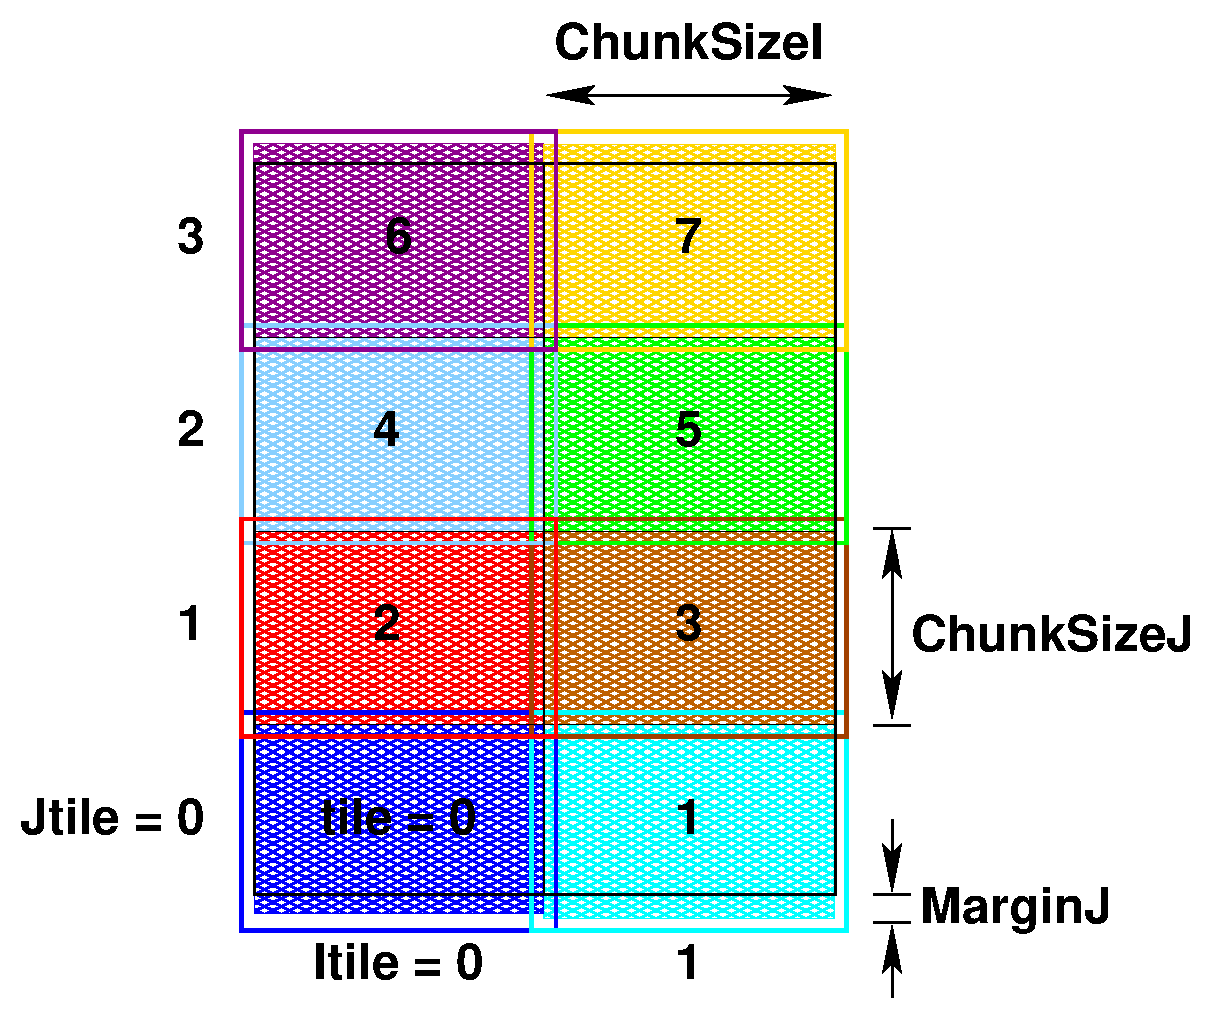
\includegraphics[height=100mm]{pics/tile3}
  \end{picture}
  \caption{A tiled grid with some ROMS tile variables.}
  \label{ftile2}
\end{figure}

The number of tiles is set in the input file as \code{NtileI}
and \code{NtileJ}. For an MPI job, the product of the two must
equal the number of MPI processes. For an OpenMP job, the
number of tiles must be a multiple of the number of threads.
For instance, for \code{NtileI}$=4$ and \code{NtileJ}$=6$, you
must have 24 MPI processes while 2, 3, 4, 6, 8, 12 and 24 are all valid
numbers of OpenMP threads. Also, a serial run could have 24
tiles and would just compute them sequentially.

Once the input file
has been read, we can compute the tile sizes in \code{get\_bounds}:
\begin{verbatim}
     ChunkSizeI = (Lm+NtileI-1)/NtileI
     ChunkSizeJ = (Mm+NtileJ-1)/NtileJ
     MarginI = (NtileI*ChunkSizeI-Lm)/2
     MarginJ = (NtileJ*ChunkSizeJ-Mm)/2
\end{verbatim}
Some internal ROMS numbers are shown in Fig.\ \ref{ftile2} and
are in the \code{BOUNDS} structure in \code{mod\_param.F}.
\code{MarginI} and \code{MarginJ} are zero if the numbers work
out perfectly, i.e.\ \code{Lm}/\code{NtileI} and
\code{Mm}/\code{NtileJ} are integers. The tile numbers match
the MPI process numbers.

In picking a numbering scheme for indices within a tile, there
are two common choices, as shown in Fig.\ \ref{fdecomp1}. Each
tile can be numbered from 1 to \code{ChunksizeI} or it can retain the
numbering it would have in the whole grid. We have chosen this
second option for ease when debugging features such as river
inputs which apply to specific locations on the grid. It is
simple to do using Fortran 90 dynamic memory allocation.

\begin{figure}[t]
\setlength{\unitlength}{10mm}
\begin{picture}(0,7)(0,0)
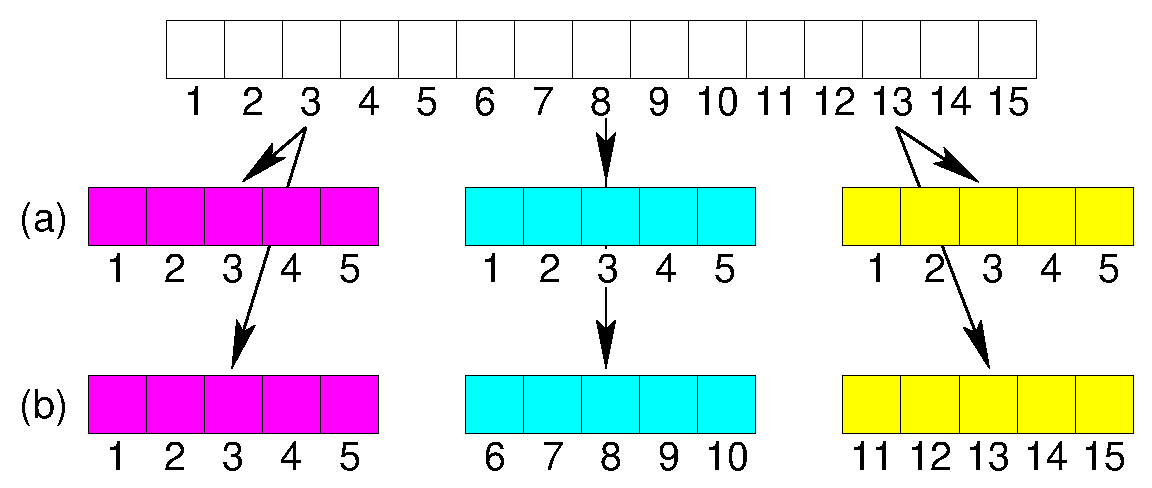
\includegraphics[width=165mm]{pics/numbering}
  \end{picture}
  \caption{A choice of numbering schemes: (a) each tile is numbered
the same, and (b) each tile retains the numbering of the parent
domain.}
  \label{fdecomp1}
\end{figure}

With the tile sizes known, we can assign beginning and ending
indices for each tile. Some of the details depend on whether or
not the domain is periodic in that direction, as shown in Fig.\
\ref{ftile3}.

\begin{figure}[tb]
\setlength{\unitlength}{10mm}
\begin{picture}(0,9)(0,0)
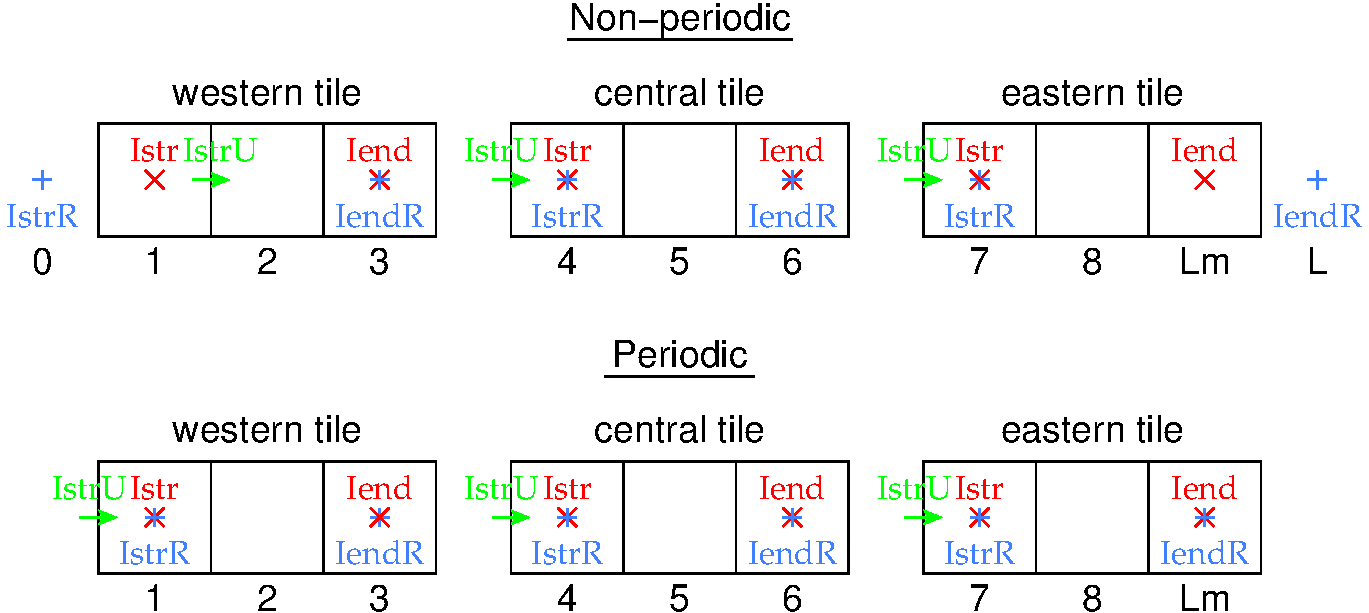
\includegraphics[width=165mm]{pics/Istr}
  \end{picture}
  \caption{Some ROMS variables for tiles, for both a periodic and
  non-periodic case. Shown are the variables in the
  \code{i}-direction, the \code{j}-direction is similar.}
  \label{ftile3}
\end{figure}

\subsubsection{MPI exchange}

For MPI jobs, the ghost points need to be updated between
interior point computations. The routines
\code{mp\_exchange2d}, \code{mp\_exchange3d} and
\code{mp\_exchange4d} can be used to update the halo points of
up to four arrays at a time. Each of these routines calls
\code{tile\_neighbors} to figure out which tiles are neighboring and
whether or not there really is a neighboring tile on each side. The
\code{mp\_exchangexd} routines then call:
\begin{verbatim}
    mpi_irecv
    mpi_send
    mpi_wait
\end{verbatim}
The exchanges happen first in the east-west direction, then in the
north-south direction, saving the need for diagonal exchanges. A figure
with interior points colored by tile and grey halo points needing an
update is shown in Fig.\ \ref{fex_2d1}(a). The updated halo points are
shown in Fig.\ \ref{fex_2d1}(b).

\begin{figure}[p]
\setlength{\unitlength}{10mm}
\begin{picture}(0,22)(-2.8,0)
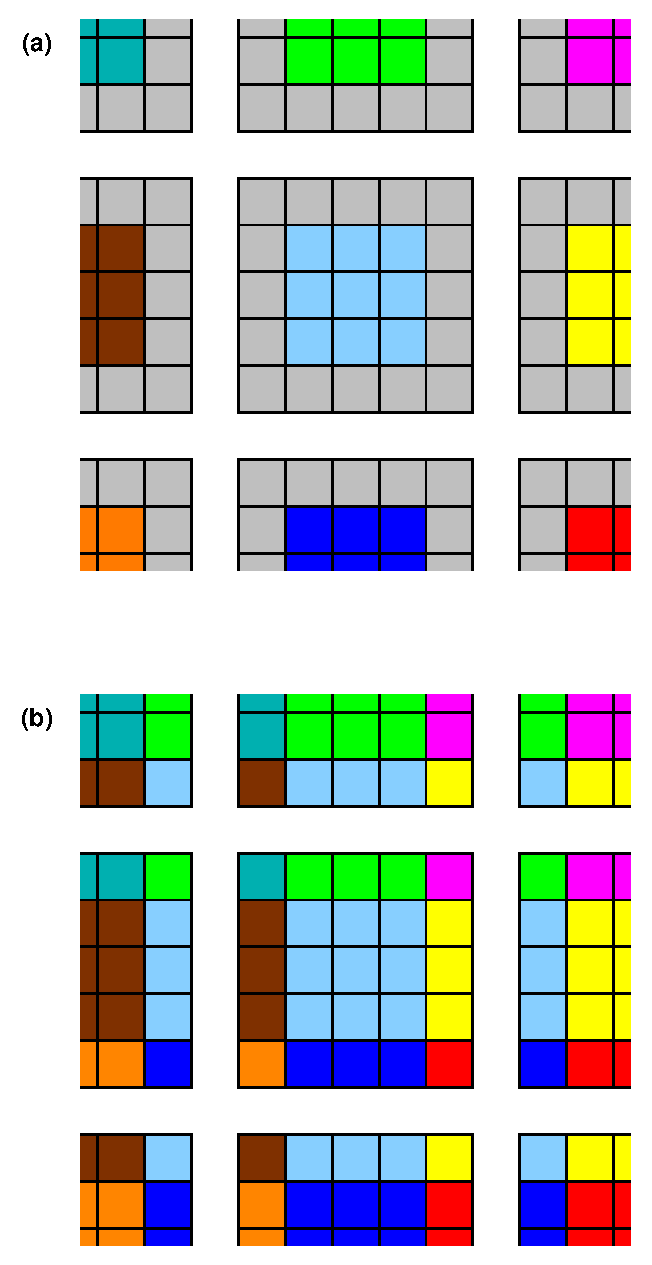
\includegraphics[height=220mm]{pics/ex_2d}
  \end{picture}
  \caption{A tiled grid with out-of-date halo regions shown in
  grey and the interior points color-coded by tile: (a) before an
  exchange and (b) after an exchange.} \label{fex_2d1}
\end{figure}

\subsubsection{Code syntax}

In \code{main3d}, many function calls are surrounded by
nesting code such as:
\begin{verbatim}
            DO ig=1,GridsInLayer(nl)
              ng=GridNumber(ig,nl)
              DO tile=first_tile(ng),last_tile(ng),+1
                CALL set_data (ng, tile)
              END DO
!$OMP BARRIER
            END DO
            IF (exit_flag.ne.NoError) RETURN
\end{verbatim}
where \code{first\_tile} and \code{last\_tile} are set in
\code{nl\_ocean.h}:
\begin{verbatim}
#if defined _OPENMP
      MyThread=my_threadnum()
#elif defined DISTRIBUTE
      MyThread=MyRank
#else
      MyThread=0
#endif
      DO ng=1,Ngrids
        chunk_size=(NtileX(ng)*NtileE(ng)+numthreads-1)/numthreads
        first_tile(ng)=MyThread*chunk_size
        last_tile (ng)=first_tile(ng)+chunk_size-1
      END DO
\end{verbatim}
\code{NtileX} and \code{NtileE} no longer depend on whether we're
using MPI:
\begin{verbatim}
      NtileX(1:Ngrids)=NtileI(1:Ngrids)
      NtileE(1:Ngrids)=NtileJ(1:Ngrids)
\end{verbatim}
Instead, \code{numthreads} varies, being set to 1 for serial jobs,
to the number of MPI processes for MPI and to
\code{omp\_get\_max\_threads()} for OpenMP jobs. For MPI jobs,
integer division gives \code{chunk\_size} the value of 1 and
\code{first\_tile} and \code{last\_tile} are both set to the process
number.

In looking at a typical routine that's called from \code{main3d},
the routine is usually quite short, calling a \code{\_tile}
version of itself in which the actual work happens:
\begin{verbatim}
    SUBROUTINE set_data (ng, tile)
    # include "tile.h"
      CALL set_data_tile (ng, tile,                        &
     &                    LBi, UBi, LBj, UBj,              &
     &                    IminS, ImaxS, JminS, JmaxS)
      RETURN
      END SUBROUTINE set_data
\end{verbatim}
Here, there are two sets of array lower and upper bounds, those
in the \code{LBi} family and those in the \code{IminS} family. Both
depend on the \code{Istr} family shown in Fig.\ \ref{ftile3}. The
\code{IminS} family is for work arrays that are local to an MPI
process or to an OpenMP thread, also local to a \code{\_tile}
routine. They are initialized:
\begin{verbatim}
      IminS=BOUNDS(ng)%Istr(tile)-3
      ImaxS=BOUNDS(ng)%Iend(tile)+3
      JminS=BOUNDS(ng)%Jstr(tile)-3
      JmaxS=BOUNDS(ng)%Jend(tile)+3
\end{verbatim}
and used:
\begin{verbatim}
      real(r8), dimension(IminS:ImaxS,JminS:JmaxS) ::  work1
      real(r8), dimension(IminS:ImaxS,JminS:JmaxS) ::  work2
\end{verbatim}
The \code{Istr} and \code{LBi} families are dimensioned by the number
of tiles once it is known by \code{inp\_par}:
\begin{verbatim}
        DO ng=1,Ngrids
          Ntiles=NtileI(ng)*NtileJ(ng)-1
          allocate ( BOUNDS(ng) % LBi  (-1:Ntiles) )
                          :
          allocate ( BOUNDS(ng) % Jend (-1:Ntiles) )
        END DO
\end{verbatim}
They are then initialized in calls to the routines in
\code{get\_bounds.F}. \code{Imin} is set to \code{-NghostPoints}
or zero, for periodic and non-periodic domains, respectively. The
\code{UBi} family is set once the \code{Istr} family is known:
\begin{verbatim}
        IF ((Itile.eq.-1).or.(Itile.eq.0)) THEN 
          LBi=Imin
        ELSE
          LBi=Istr-Nghost
        END IF
\end{verbatim}

In the case of \code{set\_data}, we are simply passing array indices
for the tiled arrays. To access the tiled arrays from within
\code{set\_data\_tile}, we need to \code{use} the relevant modules
and then refer to the array with its full name:
\begin{verbatim}
      USE mod_forces
            :
      CALL set_2dfld_tile (ng, tile, iNLM, idCfra,             &
     &                     LBi, UBi, LBj, UBj,                 &
     &                     FORCES(ng)%cloudG,                  &
     &                     FORCES(ng)%cloud,                   &
     &                     update)
\end{verbatim}
In other cases, the parent routine would have the \code{use}, then
would pass the relevant array to the \code{\_tile} routine:
\begin{verbatim}
      USE mod_grid
          :
      CALL prsgrd_tile (ng, tile,                              &
          :
     &                  GRID(ng) % Hz,                         &
          :
      SUBROUTINE prsgrd_tile (ng, tile,                        &
          :
     &                        Hz, z_r, z_w,                    &
          :
      real(r8), intent(in) :: Hz(LBi:,LBj:,:)
\end{verbatim}
This allows the \code{\_tile} routine to use \code{Hz} with the same
syntax as the pre-parallel, pre-module code once had.

\subsubsection{Input/output}

In ROMS, the distributed memory I/O is all happening on the master process
(0) unless you specifically ask it to use MPI-I/O, which requires
either or both of \code{PARALLEL\_IN} \code{PARALLEL\_OUT} and
either of the \code{HDF5} or \code{PNETCDF} \code{cpp} flags to be
defined. If you choose \code{HDF5}, you will be reading and/or writing
\code{HDF5} files and will need to update your pre- and post-processing
tools accordingly. I have tentatively tried the parallel I/O and
found it to be exceedingly slow---I've been told since that this
is the fault of the \code{NetCDF-4} layer sitting on top of
\code{HDF5}---\code{HDF5} alone should be fast.

In the case of having all the I/O pass through the master process,
we can still read and write classic NetCDF-3 files. Care must be
taken though, in the event of an error. ROMS has been cleaned up so
that the master process will broadcast its return state to the other
processes and they can all die gracefully together when there is a
problem.

An example of a routine which reads from disk is \code{get\_grid},
called from \code{initial}. Each MPI process calls \code{get\_grid}:
\begin{verbatim}
        CALL get_grid (ng, iNLM)
# ifdef DISTRIBUTE
        CALL mp_bcasti (ng, iNLM, exit_flag)
# endif
        if (exit_flag.ne.NoError) RETURN
\end{verbatim}
If any one of the processes has trouble, it will enter into the
\code{exit\_flag} which is then shared by all.

To read in an array variable, all processes in \code{get\_grid} use
\code{nf\_fread2d} and friends:
\begin{verbatim}
            status=nf_fread2d(ng, model, ncname, ncGRDid(ng),      &
     &                        var_name(it), var_id(it),            &
     &                        0, gtype, Vsize,                     &
     &                        LBi, UBi, LBj, UBj,                  &
     &                        Fscl, Fmin, Fmax,                    &
     &                        GRID(ng) % rmask,                    &
     &                        GRID(ng) % rmask)
            IF (status.ne.nf90_noerr) THEN
              exit_flag=2
              ioerror=status
              EXIT
            END IF
\end{verbatim}
Within \code{nf\_fread2d}, we get to a call to the NetCDF library
from just the master process:
\begin{verbatim}
      IF (InpThread) THEN
        status=nf90_get_var(ncid, ncvarid, wrk, start, total)
            :
      END IF
# ifdef DISTRIBUTE
      CALL mp_bcasti (ng, model, status)
# endif
      IF (status.ne.nf90_noerr) THEN
        exit_flag=2
        ioerror=status
        nf_fread2d=status
        RETURN
      END IF
\end{verbatim}
At this point, the master process has the entire 2-D array stored in
\code{wrk}. This then needs to be divvied out to the various tiles
to their copy of the array in question (stored in the \code{A}
argument to \code{nf\_fread2d}):
\begin{verbatim}
    # ifdef DISTRIBUTE
            CALL mp_scatter2d (ng, model, LBi, UBi, LBj, UBj,         &
         &                     Nghost, MyType, Amin, Amax,            &
    #  if defined READ_WATER && defined MASKING
         &                     NWpts, SCALARS(ng)%IJwater(:,wtype),   &
    #  endif
         &                     Npts, wrk, A)
\end{verbatim}
Something similar happens when writing to output files.

\paragraph{PIO}
I have a branch in which I linked to the
\href{https://github.com/NCAR/ParallelIO}{Parallel-IO} or PIO library
from NCAR. It's unstable for fewer writers than processes, but let
me know if you'd like to try it.
